%%%% Martin Rotter, Tomáš Kukučka, Jiří Zehnula - FJAA (zápisky z přednášek)
%%%%
%%%% kompilováno přes cslatex --> dvips --> ps2pdf
%%%%
%%%%%%%%%%%%%%%%%%%%%%%%%%%%%%%%%%%%%%%%%%%%%%%%%%%%%%%%%%%%%%%%%%%%%%%%%%%%%%%%%
%%%%%%%%%%%%%%%%%%%%%%%%%%%%%%%%%%%%%%%%%%%%%%%%%%%%%%%%%%%%%%%%%%%%%%%%%%%%%%%%%

\documentclass[10pt, a4paper, titlepage]{article}

\usepackage{czech}						% napsáno česky
\usepackage[utf8]{inputenc}				% napsáno v UTF-8
\usepackage[tables,figures]{upreport}	% UPOL styl
\usepackage{upstyles}
\usepackage{a4wide}
\usepackage{amsmath}
\usepackage{amssymb}
\usepackage{amsthm}
\usepackage{vaucanson-g}				% makro pro kreslení grafů a automatů
\usepackage{alltt}

\setlength{\parindent}{0pt}
\setlength{\parskip}{1ex plus 0.5ex minus 0.2ex}

\title{KMI/FJAA  -- Formální jazyky a automaty}
\author{M.~Rotter, T.~Kukučka, J.~Zehnula}
\date{\today}

\docinfo{M.~Rotter, T.~Kukučka, J.~Zehnula}{KMI/FJAA  -- Formální jazyky a automaty}

\newtheoremstyle{note}
{15pt}
{15pt}
{}
{}
{}
{:}
{.5em}
{}
\theoremstyle{note}
\newtheorem{veta}{\textbf{Věta}}
\newtheorem{definice}{\textbf{Definice}}
\newtheorem{dukaz}{\textbf{Důkaz}}
\newtheorem{priklad}{\textbf{Příklad}}
\newtheorem{poznamka}{\textbf{Poznámka}}
\newtheorem{dusledek}{\textbf{Důsledek}}
\newcommand{\ekna}{$\varepsilon$KNA} %byl jsem línej to pořád psát
\newcommand{\aut}[1]{$A_#1= \langle \Sigma,Q_#1,\delta_#1,q_{0#1},F_#1 \rangle$}

\abstract{Tento dokument je pouze přepisem zápisků a poznámek z přednášek předmětu KMI/FJAA. Přednášel \link{doc. Vilém Vychodil PhD}{http://vychodil.inf.upol.cz/}.}

\pagestyle{empty}
\makeindex

\begin{document}
\maketitle

\section{Historie}
Počátek úvah, jež byly později základem seriozního zkoumání formálních jazyků potažmo automatů se datuje do 30. let.
Průkopníkem této oblasti byl \link{Noam Chomsky}{http://cs.wikipedia.org/wiki/Noam_Chomsky}
\footnote{Jméno této osoby čti [\emph{čomski}] a zapamatuj si ke státnicím, že Chomsky byl \emph{nebezpečný levicový intelektuál}.}.

Jako příklad selhání autora programovacího jazyka si uveďme jazyk \textbf{Fortran}, jehož konstrukce byla po syntaktické stránce špatná,
což vedlo ke \textbf{gramatické ne jednoznačnosti} tohoto jazyka.

\section{Kódová analýza}
\subsection{Lexikální analýza}
Dělení kódu na tokeny\footnote{Překládej jako \emph{část, díl nebo také fráze}.}, jež se zapisují například ve stylu
$\langle\text{ znak, identifikátor }\rangle$.
Příkladem je tedy i token $\langle =, assignment \rangle$ a jiné.

\subsection{Syntaktická analýza}
Syntaktická analýza vytváří stromovou závislost jednotlivých tokenů, jejíž reprezentace se nazývá \emph{syntaktický-derivační strom}.
V rámci této analýzy rozlišme:
\begin{enumerate}
\item
Teorii jazyků, jenž se zabývá stavbou jazyka (respektive jeho syntaxí) a poskytuje tzv. \textbf{generativní aparát}.
Dodejme, že gramatika říká, v jakém tvaru může být zapsán validní program.

\item
Teorii automatů, jež poskytuje tzv. \textbf{analytický aparát}.
Dodejme, že automatem se rozumí de-facto jednoduchý algoritmus.
\end{enumerate}

\section{Základní pojmy}
\begin{itemize}
\item
\textbf{Symbol} (případně znak). Jedná se o syntaktický pojem (význam tedy nehraje roli), který představuje \emph{jméno} (analogicky k \emph{písmenu} z přirozeného jazyka).
Mezi symboly počítejme například \textbf{0, +, Š, while}.

\item
\textbf{Abeceda}. Abecedou rozumíme množinu (například množinu $X$) všech přípustných \emph{symbolů} (znaků), přičemž taková množina je neprázdná (tedy $|x|>0$) a konečná.
Konečnost množiny je omezení dané reprezentovatelností množiny v rámci počítačové techniky.
Abecedy značíme řeckými písmeny. Například $\Sigma, \Sigma^{'}, \Gamma, \ldots, \Omega$.
Například $\Sigma = \lbrace a, b, c \rbrace$.

\item
\textbf{Řetězec} (případně slovo). Jedná se o konečnou posloupnost symbolů (znaků) vybraných z nějaké dané abecedy.
Například $\langle a_{1}, a_{2}, \ldots, a_{n} \rangle \in \Sigma, n$ nazvěme \emph{délkou řetězce}.
Formálně definujme řetězec jakožto \emph{zobrazení}
$$
x : \lbrace a, b, c, d, \ldots, i, j, \ldots \rbrace \rightarrow \Sigma
$$
kde
$$
1 \rightarrow a, 2 \rightarrow b, 3 \rightarrow c
$$ a tak podobně.
Délku řetězce označme $|x|$.

\item
\textbf{Prázdný řetězec}. Jedná se o řetězec, pro který platí, že $|x| = 0$ a značíme jej $\varepsilon$, přičemž platí následující zápis:
$$
\varepsilon \subseteq \emptyset \rightarrow \Sigma
$$
Prázdný řetězec \textbf{není} symbolem, tedy $\varepsilon \notin \Sigma$.
\end{itemize}

\begin{veta}
Nad $k$-prvkovou abecedou je právě $k^{n}$ řetězců délky $n$.
\end{veta}


\begin{poznamka}
Uveďme si rovněž značení pro dva důležité pojmy:

\begin{itemize}
\item
$\Sigma^{*}$ označuje množinu všech řetězců nad abecedou$\Sigma$.

\item
$\Sigma^{+}$ označuje množinu všech řetězců nad abecedou$\Sigma$ vyjma $\varepsilon$.
\end{itemize}
\end{poznamka}

\section{Operace s řetězci}
\begin{itemize}
\item
\textbf{Zřetězení} (konkatenace). Jde v podstatě o spojení\footnote{Pro milovníky jazyka Scheme můžeme tuto operaci přirovnat k proceduře \emph{append}}
dvou řetězců v daném pořadí do jednoho řetězce.

\begin{priklad}
Mějme dva řetězce $a$, $b$:
$$
a_{1}\ldots a_{n} \text{ a } b_{1}\ldots b_{m}
$$
Pak jejich zřetězení má tvar:
$$
a_{1}\ldots a_{n}b_{1}\ldots b_{m}
$$
Identifikátorem\footnote{Identifikátor zřetězení se velmi čast v zápisech zřetězení vynechává.} operace
zřetězení je $\circ$, například $x\circ y$ je zřetězením řetězců $x$ a $y$.
Formálně takto:
\begin{gather*}
x : \lbrace 1,\ldots, n \rbrace \rightarrow \Sigma \\
y : \lbrace 1,\ldots, m \rbrace \rightarrow \Sigma \\
x \circ y : \lbrace 1,\ldots, n+m \rbrace \rightarrow \Sigma
\end{gather*}
\end{priklad}

\begin{poznamka}
Algebraicky je tatáž operace zapsána jako $\langle \Sigma^{*}, \circ, \varepsilon \rangle$.
\end{poznamka}

\item
\textbf{Rovnost řetězců}
Pro prohlášení dvou řetězců za sobě rovné v žádaném smyslu je třeba splnit obecně dvě následující podmínky:
\begin{enumerate}
\item
Oba řetězce mají stejnou délku, tedy $|x| = |y|$.

\item
Bude-li délka označena jako $n$, pak musí platit, že $\forall i | i \in \lbrace 1, \ldots, n \rbrace, x(i) = y(i)$.
Tedy každé dva k sobě náležící symboly z daných řetězců jsou si rovny.
\end{enumerate}
Uvažujeme-li rovnost řetězců, pak je záhodno uvažovat následující pojmy:
\begin{itemize}
\item
\textbf{Prefix} řetězce. Označme jej $Pfx(x) = \lbrace y | \exists z \text{ tak, že } yz = x \rbrace$.

\item
\textbf{Infix} řetězce. Označme jej $Ifx(x) = \lbrace y | \exists z_{1}, z_{2} \text{ tak, že } z_{1}yz_{2} = x \rbrace$.

\item
\textbf{Sufix} řetězce. Označme jej $Sfx(x) = \lbrace y | \exists z \text{ tak, že } zy = x \rbrace$.
\end{itemize}

\begin{veta}
\begin{gather*}
xy = xz \: \Longrightarrow \: y = z \\
yx = zx \: \Longrightarrow \: y = z
\end{gather*}
Algebraicky je operace zapsána jako $\langle \Sigma^{*}, \cdot, \varepsilon \rangle$.
\end{veta}

\begin{veta}
Vyslovme předpoklad, že platí $xy = uv$. Pak platí právě jedno z těchto tvrzení:
\begin{gather*}
x = u, y = v \\
|x| > |u| \text{ a } \exists w| w \neq \varepsilon, \text{ tak že } x = uw \text{ a } v = wy \\
|x| < |u| \text{ a } \exists w| w \neq \varepsilon, \text{ tak že } u = xw \text{ a } y = wv
\end{gather*}
\end{veta}

\item
\textbf{N-tá mocnina} řetězce.
$$
x^{n} = \left\lbrace
\begin{array}{l l}
x & \text{pro } n=1 \\
xx^{n-1} & \text{v ostatních případech} \\
\end{array}
\right\rbrace
$$
respektive
$$ x^{n} = \left\lbrace
\begin{array}{l l}
\varepsilon & \text{pro } n=0 \\
xx^{n-1} & \text{v ostatních případech} \\
\end{array}
\right\rbrace
$$
\begin{poznamka}
Mějme na paměti, že operace mocnění má vyšší prioritu než-li operace konkatenace (zřetězení).
\end{poznamka}

\begin{veta}
Mějme $u \text{ a } v \in \Sigma^{*}$, pak platí $uv = vu$ (komutativita), právě
tehdy, když $\exists z| z \in \Sigma^{*} \text{ a nezáporná celá čísla } p, q \text{ tak, že } u = z^{p} \text{ a } v=z^{q}$.
\end{veta}

Předpokládejme, že po $p, z, q$ máme $u = z^{p}, v = z^{q}$. Pak obecně platí následující zápis:
$$
uv = z^{p}z^{q} = z^{p+q} = z^{q} z^{p} = vu
$$

Předpokládejme, že $uv = vu$. Indukcí přes $|uv|$ předpokládáme, že tvrzení platí pro libovolné dva řetězce, jejichž délka zřetězení je menší
než-li $|uv|$. Mohou nastat tyto případy:
\begin{enumerate}
\item
$|u| = |v|, \text{ pak } u = v, \text{ pak } z = u, p = q = 1$

\item
$|u| < |v|$
\end{enumerate}

Berme v potaz také následující zápis doplněný obrázkem: \ref{obr-1}

\begin{gather*}
uw = v \\
wu = v \\
uw = wu \\
|uw| < |uv|, \text{ tedy } \exists z, p, q  \text{ tak, že } u = z^{p}, w = z^{q}, v = z^{p+q}
\end{gather*}

\begin{figure}[ht]
\centering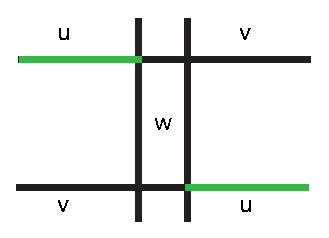
\includegraphics[width=5cm]{dukaz-1.eps}
\caption{Grafické znázornění komutativity zřetězení řetězců.}\label{obr-1}
\end{figure}
\end{itemize}

\section{Formální jazyk}
Zaveďme si pojem \emph{formální jazyk nad množinou všech řetězců} $\Sigma^{*}$. Označme tento jazyk jako $L$. Pak platí tato tvrzení:
\begin{eqnarray*}
L &\subseteq& \Sigma^{*} \text{ (každá podmnožina abecedy je jazykem)} \\
L &=& \emptyset \text{ (prázdný jazyk)} \\
L &=& \lbrace \varepsilon \rbrace \text{ (jazyk s prázdným řetězcem)} \\
L &=& jazyk C++ \text{ (jazyk C++)} \\
&\vdots&
\end{eqnarray*}
\textbf{Pozor, obecně platí že prázdný jazyk $\neq$ jazyk s prázdným řetězcem.}
	
\section{Lexikografické uspořádání}
Předpokládejme uspořádání na množině $\Sigma^{*}$.
Nazvěme toto uspořádání \emph{striktním totálním}. Pak toto uspořádání například pro $\Sigma = \lbrace a_{1}, \ldots, a_{n} \rbrace$
je $a_{1} < a_{2} < a_{3} < \ldots < a_{n}$.

Totální striktní uspořádání označme $<_{l}$.

Položme $x <_{l} y$ pro $x,y \in \Sigma^{*}$. To ale platí pokud platí alespoň jedno z následujících dvou tvrzení:
\begin{enumerate}
\item
$|x| < |y|$

\item
$|x| = |y| \text{ a } \exists i \text{ tak, že } x(i) < y(i) \text{ a zároveň } x(j) = y(j) \text{ pro } \forall j |j < i$
\end{enumerate}

\begin{priklad}
$\Sigma = \lbrace 0, 1 \rbrace$. Triviálně tedy $0 < 1$.
Následně striktně $\varepsilon <_{l} 0 <_{l} 1 <_{l} 00 <_{l} 01 <_{l} 10 <_{l} 11$.
\end{priklad}

\begin{veta} \label{veta-1}
Striktní totální uspořádání je asymetrické a tranzitivní. A pro $x \neq y$ platí buď $x <_{l} y$ nebo $y <_{l} x$.
\end{veta}

\begin{dusledek}
Důsledkem věty \ref{veta-1} je tvrzení, že množina $\Sigma^{*}$ je spočetně nekonečná. Dodejme, že jazyk je (obvykle) spočetná množina.
\end{dusledek}

\section{Operace nad jazyky}
\nextoutline{Mnozinové}

\subsection{Množinové}
Množinové operace nad jazyky jsou prakticky totožné operacím na kterýchkoliv jiných množinách. Můžeme tedy použít množinový průnik, sjednocení, komplement (doplněk) nebo rozdíl.

\subsection{Ostatní}
\begin{itemize}
\item
\textbf{Zřetězení} (produkt) množin. Vyjádřeme produkt takto:
$$
L_{1}L_{2} = \lbrace xy | x \in L_{1}, y \in L_{2} \rbrace
$$
Produkt množin není obecně komutativní, ale je asociativní, přičemž prázdná množina tuto operaci anihiluje.
Uveďme si rovněž monoid $\langle 2^{\Sigma^{*}}, \circ, \lbrace \varepsilon \rbrace \rangle$.

\item
\textbf{Mocnina} jazyka. Mocninu vyjádříme takto:
$$
L^{n} = \left \lbrace
\begin{array}{l l}
\lbrace \varepsilon \rbrace & \text{ pro } n = 0 \\
LL^{n-1} & \text{ pro } n \geq 1 \\
\end{array}
\right.
$$

\item
\textbf{Kleeneho\footnote{\link{Stephen Cole Kleene}{http://en.wikipedia.org/wiki/Stephen_Cole_Kleene} je známý matematik, jenž se významně podílel na položení základů teoretických počítačových věd.}} uzávěr neboli \textbf{iterace}. Tento uzávěr vyjádříme takto:
$$
L^{*} = \bigcup_{i = 0}^{\infty} L^{i}
$$

\item
\textbf{Pozitivní} uzávěr neboli pozitivní iterace. Tento uzávěr vyjádříme takto:
$$
L^{+} = \bigcup_{i = 1}^{\infty} L^{i}
$$
Všimněte si podobností mezi těmito dvěma uzávěry. Pozitivní uzávěr vynechává prázdný řetězec.

\end{itemize}

\section{Gramatiky}
Jak víme, tak jazyky mohou být \emph{nekonečné} ve smyslu, že obsahují nekonečný počet slov.
Nabízí se tedy otázka, jak tyto jazyky rozumně popsat, jak je reprezentovat resp. jak vytvořit \emph{konečnou}
sadu pravidel, jejichž aplikace by vedla k opětovné generaci původního jazyka.

\nextoutline{Prepisovací generovací pravidla}
\subsection{Přepisovací generovací pravidla}
Pravidlem rozumíme zpravidla každou takto definovanou dvojici.
$$
\langle x,y \rangle \in \Sigma^{*} \times \Sigma^{*}
$$
Pak neformálně tvrdíme, že $x$ \emph{se přepisuje} na $y$.
Nutno dodat, že předchozí zápis lze zapsat i například takto.
$$
x \rightarrow y\text{, kde symbol } \rightarrow \notin \Sigma \text{ můžeme prohlásit za tzv. metasymbol.}
$$
\subsubsection{Vlastnosti pravidel}
\begin{itemize}
\item \emph{Nezkracující} pravidlo je pravidlo, o kterém platí, že $|x| \leq |y|$. Tedy aplikaci tohoto pravidla na vstupní řetězec určitě nevznikne řetězec kratší, než-li jeho předloha.

\item $\varepsilon$ - pravidlo je pravidlo tvaru $x \rightarrow \varepsilon$.
\end{itemize}

\nextoutline{Priklady pravidel}
\subsubsection{Příklady pravidel}
\begin{priklad}
Mějme zadání abecedy $\Sigma = \lbrace a,b,c \rbrace$. Pravidla s využitím této abecedy by mohla být například tato.
\begin{eqnarray*}
aa &\rightarrow& bc \\
bb &\rightarrow& abba \\
c &\rightarrow& \varepsilon
\end{eqnarray*}
\end{priklad}

\begin{priklad}
Mějme další zadání abecedy $\Sigma = \lbrace expr, +, \times \rbrace$. Pravidla s využitím této abecedy by mohla být například tato.
\begin{eqnarray*}
\textit{expr} &\rightarrow& \textit{expr} + \textit{expr} \\
\textit{expr} &\rightarrow& \textit{expr} \times \textit{expr}
\end{eqnarray*}
\end{priklad}

\nextoutline{Prime odvozovani rezezcu pomoci pravidel}
\subsubsection{Přímé odvozování řetězců pomocí pravidel}
Uvažujme odvozovací pravidlo $ x \rightarrow y \text{ nad abecedou } \Sigma$, pak řekneme, že řetězec \emph{v} \textbf{je přímo odvozen}
z řetězce \emph{u} pomocí pravidla $ x \rightarrow y $, pokud $\exists p, q \in \Sigma^{*}$ tak, že
\begin{gather*}
u = p x q \\
v = p y q
\end{gather*}

Značení předchozí operace je následující:
$$
u \Rightarrow_{x \rightarrow y} v
$$
Slovně bychom tento zápis vystihli jako \uv{přímý přepis dle pravidla $x \rightarrow y$.}

Řetězec $v$ vznikne přímým přepisem z $u$ pomocí pravidel $P \subseteq  \Sigma^{*} \times \Sigma^{*}$, pokud
$\exists \pi \in P \text{ tak, že } u \Rightarrow_{\pi} v$.

Značme $u \Rightarrow_{P} v$. $P$ je množinou užitých pravidel. $P$ i $\Rightarrow_{p}$ jsou binární relace na $\Sigma^{*}$ a
$P \subseteq  \Rightarrow_{p}$, tedy \uv{P je podmnožinou šipky p.} Platí, že $x \rightarrow y \in P$ a $x \Rightarrow_{x \rightarrow y} y$.

\begin{priklad}
Mějme abecedu $\Sigma = \lbrace a, b, c \rbrace$ a soubor pravidel $P = \lbrace aa \rightarrow bc, a \rightarrow cab, bb \rightarrow \varepsilon \rbrace$\label{priklad-1}.
Pak by odvození v jednom kroku mohla vypadat například takto:
\begin{gather*}
baaa \rightarrow bbca \\
bac \rightarrow bcabc
\end{gather*}
\end{priklad}

\begin{definice}
Definujme pojem \textbf{derivace}. Jedná se o posloupnost řetězců ve tvaru:
$$
x_{0}, \ldots, x_{k},\text{ kde } k \geq 0\text{ a kde } \lbrace x_{0}, \ldots, x_{k} \rbrace \in \Sigma^{*}
$$
se nazývá \textbf{P-derivace délky k}, pokud $x_{i-1} \Rightarrow_{p} x_{i}, \forall 1 \leq i \leq k $.
Symbolicky totéž $x_{0} \Rightarrow_{p} x_{1} \Rightarrow_{p} \ldots \Rightarrow_{p} x_{k}$. Počet odvození tedy značí \emph{délku} derivace.
\end{definice}

Pokud pro $u, v \in \Sigma^{*} \quad \exists \text{ P-derivace } u = x_{0} \ldots x_{k} = v$, pak říkáme, že $v$ je odvozeno z $u$ pomocí pravidel z $P$, což značíme
například $u \Rightarrow_{P}^{*} v$, tímto je pochopitelně myšleno odvození ve více krocích. Platí, že $P \subseteq \Rightarrow_{P} \subseteq \Rightarrow_{P}^{+}$.

\begin{priklad}
Mějme abecedu $\Sigma = \lbrace a, \ldots, z \rbrace$ a pravidla stejná jako v příkladu \ref{priklad-1}.
Nyní odvozujeme například takto:
$$
b\underline{aa}a, \underline{bb}ca, c\underline{a}, c\underline{cab}
$$
\end{priklad}

\subsection{Formální gramatiky}
Mějme následující entity:
\begin{itemize}
\item $\Sigma$ - abeceda terminálních symbolů (tyto symboly tvoří řetězce daného jazyka).
\item $N$ - abeceda neterminálních symbolů (tyto symboly se užívají k řízení průběhu odvozování).
\end{itemize}

Dodejme, že obě množiny by měly být neprázdné a konečné.

\begin{definice}
Odvozovací pravidlo $x \rightarrow y$ se nazývá \emph{generativní}, pokud \emph{x} obsahuje alespoň jeden neterminální symbol.
\end{definice}

\begin{definice}
Mějme strukturu $G = \langle N, \Sigma, P, S \rangle$, kde $N$ je abecedou neterminálních symbolů, $\Sigma$ je abecedou terminálních symbolů,
$P$ je množinou odvozovacích pravidel a $S \in N$\hyplabel{terminal} je tzv. \emph{počátečním} resp. \emph{startovním} neterminálem. Pak tuto čtveřici nazveme \textbf{gramatikou}.
\end{definice}

\begin{poznamka}
Pokud chceme vyjádřit, že z jednoho symbolu odvozujeme několik možných alternativ, tak to zapíšeme místo klasického dlouhé zápisu
$y \rightarrow x_{1}, y \rightarrow x_{2}, \ldots$ pomocí zkrácené notace např. $y \rightarrow x_{1}|x_{2}|\ldots$
\end{poznamka}

\begin{priklad}
Gramatika může vypadat třeba takto:
\begin{eqnarray*}
N &=& \lbrace \varepsilon, S, D, I \rbrace \\
\Sigma &=& \lbrace 0, \ldots, 9, +, - \rbrace \\
P &=& \lbrace S \rightarrow -I|+I|I, I \rightarrow DI|D, D \rightarrow 0|1|\ldots |9 \rbrace \\
G &=& \langle N, \Sigma, P, S \rangle
\end{eqnarray*}
\end{priklad}

\begin{priklad}\label{priklad-2}
Nebo takto:
\begin{eqnarray*}
N &=& \lbrace S, X, Y \rbrace \\
\Sigma &=& \lbrace a, b, c \rbrace \\
P &=& \lbrace S \rightarrow XcYcX, X \rightarrow aX, X \rightarrow bX, X \rightarrow cX, X \rightarrow \varepsilon,
Y \rightarrow abY, Y \rightarrow ab \rbrace \\
G &=& \langle N, \Sigma, P, S \rangle
\end{eqnarray*}
\end{priklad}

\begin{definice}
Každý řetězec $x \in (N \cup\Sigma)^{*}$, pro který platí $S \rightarrow^{*} x$, je \textbf{větná forma} gramatiky $G = \langle N, \Sigma, P, S \rangle$.
Větná forma se nazývá \textbf{větou}, pokud $x \in \Sigma^{*}$.
\end{definice}

\begin{definice}
Jazyk generovaný gramatikou definujme jako:
$$
L(G) = \lbrace x \in \Sigma^{*} | S \Rightarrow_{G}^{*} x \rbrace
$$
Vidíme tedy, že takový jazyk obsahuje \emph{věty}, které lze odvodit ze startovacího neterminálu pomocí pravidel této gramatiky.
\end{definice}

\begin{priklad}
Tento příklad čerpá gramatiku z příkladu \ref{priklad-2}.
\begin{eqnarray*}
S &\Rightarrow_{G}^{*}& abbccYcX \\
S &\Rightarrow_{G}^{*}& Xcababababc \\
S &\Rightarrow_{G}^{*}& cYcbaX \\
S &\Rightarrow_{G}^{*}& abbccabca \\
S &\Rightarrow_{G}^{*}& cabababc
\end{eqnarray*}
\end{priklad}

\begin{definice}
Gramatiky $G_{1}$ a $G_{2}$ jsou \textbf{ekvivalentní}, pokud generují stejný jazyk.
\end{definice}

\subsection{Hierarchie gramatik}
\begin{itemize}
\item
\textbf{Gramatiky typu 0} -- jedná se o gramatiky bez omezení.

\item
\textbf{Gramatiky typu 1\label{gram-1}} -- jedná se o tzv. \emph{kontextové} nebo \emph{kontextově závislé} gramatiky.
Ty splňují následující omezení na tvar pravidel. Pro každé pravidlo gramatik tohoto typu platí, že:
\begin{enumerate}
\item
Buď je (pravidlo) ve tvaru $pAq \rightarrow p \times q, \text{ kde } p, q \in (\Sigma \cup N)^{*}, A \in N, x \in (\Sigma \cup N)^{*}$, kde \emph{p} a \emph{q}
se nazývají levým resp. pravým \textbf{kontextem}.

\item
Nebo je (pravidlo) ve tvaru $S \rightarrow \varepsilon$, kde $S$ je \emphref{startovní terminál}{terminal} gramatiky, ale pouze
za předpokladu, že $S$ se nevyskytuje na pravé straně žádného pravidla.
\end{enumerate}

Zároveň platí pro každé pravidlo (s výjimkou pravidla $S \rightarrow \varepsilon$), že délka odvozeného řetězce je minimálně stejně velká jako délka vstupního řetězce. Gramatika tedy zároveň obsahuje pouze tzv. \emph{nezkracující} pravidla.

\item
\textbf{Gramatiky typu 2} -- jedná se o tzv. \emph{bezkontextové} gramatiky, jenž obsahují pravidla ve tvaru:
$$
A \rightarrow x, \text{ kde } A \in N, x \in (\Sigma \cup N)^{*}
$$
Na levých stranách pravidel tedy očekáváme pouze neterminální symbol a na pravé straně očekáváme minimálně jeden symbol (s výjimkou pravidla $S \rightarrow \varepsilon$). $S$ se navíc nesmí vyskytovat na pravých stranách pravidel.

\begin{priklad}
Mějme tuto gramatiku:
\begin{eqnarray*}
G &=& \langle N, \Sigma, P, S \rangle \\
N &=& \lbrace A, S \rbrace \\
\Sigma &=& \lbrace 0, 1 \rbrace \\
P &=& \lbrace S \rightarrow 0A, A \rightarrow \varepsilon \rbrace
\end{eqnarray*}
\end{priklad}

\item
\textbf{Gramatiky typu 3\label{gram-3}} -- jedná se o tzv. \emph{regulární} resp. \emph{pravolineární} gramatiky, které obsahují pravidla ve třech následujících tvarech:

\begin{enumerate}
\item
$A \rightarrow bB, \text{ kde } A,B \in N, b \in \Sigma$

\item
$A \rightarrow a$

\item
$S \rightarrow \varepsilon$
\end{enumerate}

\end{itemize}

\begin{poznamka}
Každý konečný jazyk je regulární.
\end{poznamka}

\begin{dukaz}
Mějme jazyk $L = \lbrace x_{1},\ldots, x_{n} \rbrace$. Abychom tento jazyk prohlásili za regulární, tak je třeba najít regulární gramatiku,
která tento jazyk generuje.

Mějme tedy nějaké dané $\Sigma \text{ a } S$ a zvolme \emph{N}. Následně platí $\forall x_{i} \in L$ je dvojího typu:

\begin{enumerate}
\item
$x_{i} = \varepsilon \text{ a následně } S \rightarrow \varepsilon$

\item
$x_{i} = a_{1}\ldots a_{k} \text{ a následně } S \rightarrow a_{i1}A^{'}, A^{'} \rightarrow a_{i2}A^{''},\ldots\ldots, A^{k-1} \rightarrow a_{ik}A^{k}$
\end{enumerate}
\end{dukaz}

\begin{figure}[ht]
\centering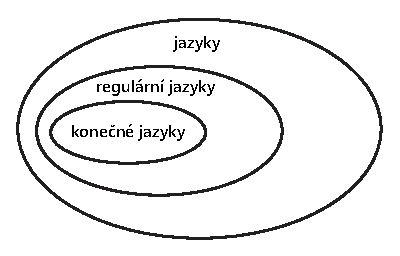
\includegraphics[width=8cm]{vajicko-1.eps}
\caption{Vychodilovo \uv{vajíčko.}}\label{obr-2}
\end{figure}

\vspace{30px}

\begin{priklad}
\begin{eqnarray*}
N &=& \lbrace S \rbrace \\
\Sigma &=& \lbrace a, b \rbrace \\
P &=& \lbrace S \rightarrow aSb | \varepsilon \rbrace \\
L(G) &=& \lbrace a^{n}b^{n} | \quad n \geq 0 \rbrace
\end{eqnarray*}
Máme tedy \emph{bezkontextový} jazyk.
\end{priklad}

\begin{priklad}
\begin{eqnarray*}
N &=& \lbrace S \rbrace \\
\Sigma &=& \lbrace a, b \rbrace \\
P &=& \lbrace S \rightarrow SS|aSb|bSa| \varepsilon \rbrace
\end{eqnarray*}
$L(G)$ je \emph{bezkontextový} jazyk.
\end{priklad}

\begin{priklad}
\begin{eqnarray*}
N &=& \lbrace S, V \rbrace \\
\Sigma &=& \lbrace p,),(, \Rightarrow, ! \rbrace \\
P &=& \lbrace S \rightarrow V|(S \Rightarrow S)|!S, V \Rightarrow pV|p \rbrace
\end{eqnarray*}
$L(G)$ je jazyk všech výrokových formulí.
\end{priklad}

%%%%%%%%%%%%%%%%%%%%%%%%%%%%%%%%%%%%%%
%%%%%%%%%%%%%%%%%%% 3. a 4. přednáška - Tom


\subsection{Gramatika nezkracující}
Gramatika G se nazývá nezkracující, pokud má pouze nezkracující pravidla a může mít pravidlo ve tvaru $S \rightarrow \varepsilon$, přičemž $S$ se nenachází na žádné z pravých stran.

\begin{priklad}
\begin{eqnarray*}
N &=& \lbrace S, A, B, C\rbrace \\
\Sigma &=& \lbrace a, b, c\rbrace \\
P &=& \lbrace S \rightarrow \varepsilon |abc|Ac, A \rightarrow aBcb, Bcb \rightarrow bBc, Bcc \rightarrow Ccc, bc \rightarrow Cb, aC \rightarrow aab|aA \rbrace
\end{eqnarray*}
\end{priklad}

\begin{veta}
Gramatiky typu 1(\ref{gram-1}) a 3(\ref{gram-3}) jsou nezkracující.
\end{veta}

\begin{veta}
Ke každé gramatice $G$, existuje ekvivalentní gramatika $G^{'}$, ve které jsou všechna pravidla obsahující terminální symboly ve tvaru $A \rightarrow a$, kde $A \in N, a \in \Sigma$.
\end{veta}

\begin{dukaz}
Pro každý terminál $a \in \Sigma$, zavedeme terminál $N_{a}$ a pravidlo $N_{a} \rightarrow a$.
Všechny výskyty terminálů ve výchozích pravidlech nahradíme příslušnými pomocnými neterminály.
$$
Bcb \rightarrow bBc \text{ se změní na } BN_{c}N_{b} \rightarrow N_{b} BN_{c}, 
N_{c} \rightarrow c, N_{b} \rightarrow b
$$
\end{dukaz}

\begin{veta}
Ke každé nezkracující gramatice existuje ekvivalentní gramatika, která je kontextově \emph{závislá}.
\end{veta}

\begin{dukaz}
Předpokládejme, že $G = \langle N, \Sigma, P, S \rangle$ je nezkracující gramatika. Dle věty 7 můžeme předpokládat, 
že všechna pravidla jsou buď ve tvaru $A \rightarrow a$ (nevadí) nebo ve tvaru obecně. 
$A_{1} A_{2} \cdots A_{m} \rightarrow B_{1} B_{2} \cdots B_{n}$, kde $A_{1}, \ldots,A_{m}, B_{1}, \ldots,B_{n} \in N$ a navíc $m \leq n$. 
Tj. taková pravidla lze psát ve tvaru $A_{1} A_{2} \cdots A_{m} \rightarrow B_{1} B_{2} \cdots B_{my}$, kde $y = B_{m+1} \cdots B_{n}$ 
Budeme uvažovat nové pomocné neterminály $X_{1},...,X_{m}$ \footnote{pro každé pravidlo se uvažují zvlášť}. 
A zavedeme následující pravidla:
\begin{gather*}
A_{1} A_{2} \cdots A_{m} \rightarrow X_{1} A_{2} \cdots A_{m} \\
X_{1} A_{2} \cdots A_{m} \rightarrow X_{1} X_{2} A_{3} \cdots A_{m} \\
\vdots \\
X_{1} X_{2} \cdots X_{m-1} A_{m} \rightarrow X_{1} \cdots X_{m-1} X_{my} \\
X_{1} X_{2} \cdots X_{my} \rightarrow B_{1} X_{2} X_{3} \cdots X_{my} \\
\vdots \\
B_{1} B_{2} \cdots B_{m-1} X_{my} \rightarrow B_{1} B_{2} \cdots B_{m-1}B_{my}
\end{gather*}
Tento postup se aplikuje pro všechna pravidla. Hledaná gramatika $G^{'}$ se skládá z $\Sigma, N$ + všechny pomocné terminály + všechna odvozená pravidla.
\end{dukaz}

\subsection{Základní vlastnosti bezkontextových gramatik}
\begin{itemize}		%% Je to dostatečně vyčerpávající?
\item
Levé strany pravidel obsahují jediný neterminál.

\item
Odvozování nezávisí na kontextu.

\end{itemize}

\begin{veta}
Mějme bezkontextovou gramatiku  $G = \langle N, \Sigma, P, S \rangle$ a nechť $X_{1} \cdots X_{k}, \ldots, z$ 
je P-derivace délky $n$, kde $X_{1}, \ldots, X_{k} \in (N \cup \Sigma)$ a $z \in (N \cup \Sigma)^{*}$ 
a potom pro každé $i = 1, \ldots, k$  existuje řetězec $z_{i} \in (N \cup \Sigma)^{*}$ 
a P-derivace $X_{i}, \ldots, z_{i}$ délky $n_{i}$ tak, že $z = z_{1} ,z_{2}, \ldots, z_{k}$ a $n = n_{1} + n_{2} + \cdots + n_{k}$
\end{veta}

\begin{dukaz}
Tvrzení prokážeme indukcí přes délku výchozí derivace $X_{1} \cdots X_{k}, \ldots, z$.
Pro $n = 0$: Triviální $z = X_{1} \cdots X_{k}, z_{i} = X_{i}, n_{i} = 0$. Každé $X_{i}$ je derivace délky $0$. 
Nechť tvrzení platí pro libovolnou derivaci délky $n$ a dokážeme, že $X_{1} \cdots X_{k}$ je P-derivace délky $n + 1$.
Jelikož má uvažovaná P-derivace délku n + 1, lze ji psát ve tvaru:
$$
X_{1} \cdots X_{k}, \ldots, y \footnote{$X_{1} \cdots X_{k}, \ldots$, y má délku n}, z 
$$
Máme $y \Rightarrow_{G}z$. Můžeme aplikovat indukční předpoklad:
Existují řetězce $y_{1}, \ldots, y_{k}$ a P-derivace $X_{1}, \ldots, y_{1}$ až $X_{k}, \ldots, y_{k}$ 
délek $n_{1} \cdots n_{k}$ tak, že $y = y_{1} y_{2} \cdots y_{k}$ a $n = n_{1} + n_{2} + \cdots + n{k}$. 
Z faktu, že $y  \Rightarrow_{G}z$ a z toho, že gramatika je bezkontextová plyne, že $y$ je ve tvaru 
$y = y^{''} y^{'} A w^{'} w^{''}$ pro $i = 1, \ldots, k$. Pak $z$ je ve tvaru $z = y^{''} y^{'} u w^{'} w^{''}$ a $A \rightarrow n \in P$,
to jest $X_{i}, \ldots, y_{i}, y^{'} u w^{'}$ je P-derivace délky $n_{i+1}$. Hledané derivace jsou:
\begin{gather*}
X_{1}, \ldots, y_{1} \\
\vdots \\
X_{i-1}, \ldots, y_{i-1} \\
X_{i}, \ldots, y_{i} y^{'} u w^{'} \\
X_{1+1}, \ldots, y_{i+1} \\
X_{k}, \ldots, j_{k} \\ %% zkontrolovat!!!
\end{gather*}
\end{dukaz}

\begin{priklad}
\begin{eqnarray*}
N &=& \lbrace S \rbrace \\
\Sigma &=& \lbrace a, b \rbrace \\
P &=& \lbrace S \rightarrow SS|aSb|bSa| \varepsilon \rbrace
\end{eqnarray*}
Posloupnost: $SbSaS, SbSa, SbaSba, aSbbaSba , abbaSba$ je P-derivace délky 4. \\*
Hledáme P-derivace:
\begin{enumerate}
\item
$S, aSb, ab$ (délka 2)
\item
$b$ (délka 0)
\item
$S, aSb$ (délka 1)
\item
$a$ (délka 0)
\item
$S, \varepsilon $ (délka 1)
\end{enumerate}
\end{priklad}

\begin{priklad}
Gramatika s jediným pravidlem $aBc \rightarrow abc$
\end{priklad}

\begin{poznamka}
U regulárních a kontextových gramatik lze hned vidět, jestli $\varepsilon \in L(G)$.
\end{poznamka}

Pro bezkontextovou gramatiku $G = \langle N, \Sigma, P,S \rangle$ zavedeme následující podmnožiny
\begin{gather*}
E_{0} = \lbrace A \in N | A \rightarrow \varepsilon \in P \rbrace \\
E_{i+1} = E_{i} \cup \lbrace A \in N | A \rightarrow x, \text{ kde } x \in E_{i}^* \rbrace
\end{gather*}

\begin{priklad}
\begin{eqnarray*}
A &\rightarrow& \varepsilon \\
B &\rightarrow& \varepsilon \\
E_{0} &=& \lbrace A, B \rbrace \\
E_{1} &=& \lbrace A, B, F \rbrace \\
E_{2} &=& \lbrace A, B, F, G \rbrace
\end{eqnarray*}
$$
E_{i} \subseteq N, E_{N} = \bigcup_{i=0}^{\infty} E_{i}
$$
Jelikož je $N$ konečná, musí platit:
\begin{gather*}
E_{0} \subseteq E_{1} \subseteq E_{2} \subseteq \cdots \subseteq E_{i} = E_{i+1} = E_{i+2} \\
E_{N} = E_{i}
\end{gather*}
\end{priklad}

\begin{veta}
Pro každou bezkontextovou gramatiku $G = \langle N, \Sigma, P,S \rangle$ a pro příslušné $E_{N}$ platí následující $A \Rightarrow_{G}^{*}\varepsilon$, pak $A \in E_{N}$. 
Speciálně $\varepsilon \in L(G)$, pak $S \in E_{N}$.
\end{veta}

\begin{dukaz}
Prokážeme obě implikace: \\
Pokud $A \Rightarrow_{G}^{*}\varepsilon$, pak prokážeme indukci přes délku P-derivace, tj. triviální případ je $A \Rightarrow_{G}\varepsilon$, 
tj. existuje pravidlo $A \rightarrow \varepsilon \in P$ tj. $A \in E_{0}$.
Předpokládejme, že tvrzení platí pro všechny P-derivace délky $n$.
Mějme $A, \ldots, \varepsilon$ P-derivace délky n + 1. Použitím předchozí věty $(A, X_{1} \cdots X_{k}, \ldots, \varepsilon)$ $A, X_{i} \cdots X_{n}, \ldots, \varepsilon$.
Tzn. existují derivace $X_{i}, \ldots, \varepsilon$ délek nejvýše $n$. Z předpokladu $X_{i} \in E_{n}$, pro každé $i$ tj. i $A \in E_{N}$. 
$\Leftarrow$ Dokáže, že pro každé $E_{i}$ platí, pokud $E \in E_{i}$ pak $A \Rightarrow_{G}^{*}\varepsilon$. Pro $E_{0}$ zřejmé.
$A \rightarrow X_{0} \cdots X_{k}, A \in E_{j}$.
\end{dukaz}

\begin{veta}
Pro každou bezkontextovou gramatiku $G$, existuje bezkontextová gramatika $G^{'}$ neobsahující $\varepsilon$ pravidla tak, že $L(G) \setminus \lbrace \varepsilon \rbrace = L(G^{'})$.
\end{veta}

\begin{dukaz}
$G = \langle N, \Sigma, P,S \rangle$ - výchozí gramatika.\\
Stanovíme množinu $E_{n}$ dle předchozího postupu $G^{'} = \langle N, \Sigma, P^{'},S \rangle$.
$P^{'} = \lbrace A \rightarrow y|A \rightarrow x \in P$ a $y \in D_{(x)} \rbrace$, kde $D_{(x)}$ značí množinu řetězců, které jsou neprázdné 
a vznikly z řetězce $x$ vynecháním libovolného množství neterminálů z $E_{N}$.
\end{dukaz}

\begin{priklad}
\begin{eqnarray*}
E_{n} &=& \lbrace A, B \rbrace \\
X &\rightarrow& aAbAB \\
&\ldots& \\
X &\rightarrow& aAbAB \\
X &\rightarrow& abAB \\
X &\rightarrow& aAbB \\
X &\rightarrow& aAbB \\
X &\rightarrow& aAbA \\
X &\rightarrow& abB \\
X &\rightarrow& abA \\
X &\rightarrow& aAb \\
X &\rightarrow& ab
\end{eqnarray*}
\end{priklad}

\begin{veta}
Pro každou bezkontextovou gramatiku existuje ekvivalentní bezkontextová gramatika, která je navíc kontextová (a tudíž nezkracující)
\end{veta}

\begin{dukaz}
Vstupní gramatika $G$. Dle předchozí věty existuje $G^{'}$ tak, že $L(G) \setminus \lbrace \varepsilon \rbrace = L(G^{'})$. 
$G^{'}$ je nezkracující a kontextová, protože nemá $\varepsilon$ pravidla. Pokud $\varepsilon$ nepatří do $L(G)$, pak jsme hotovi.
Pokud $\varepsilon \in L(G)$. Pak $G^{'}$ rozšíříme tak, že přidáme startovní symbol $S^{'}$ 
a pravidlo $S^{'} \rightarrow \varepsilon$ a $S^{'} \rightarrow S$.
\end{dukaz}
dopsat jednu stránku

% 4. přednáška
\section{Automaty}
Gramatiky x automaty

generativní formalismus

Automaty - analytické formalismy

Konečné automaty: neformální
výpočetní formalismus \uv{jednoduchý počítač}
omezená paměť
vstup: řetězec nad vstupní abecedou $\Sigma.$ Řídící jednotka. Skládá se z konečně mnoha stavů.
\textbf{Počátek činnosti:} Vstup = celý vstupní řetězec. Řídící jednotka je v počátečním (iniciálním) stavu.
\textbf{Činnost automatu:} Na základě prvního symbolu na vstupu a na základě aktuálního stavu se řídící jednotka 
přepne do jiného stavu a odebere vstupní symbol.\\
\textbf{Konec činnosti:} Byl přečten celý vstupní řetězec. Podle toho v jaké končí automat stavu říkáme, 
že buď přijímá nebo zamítá vstupní řetězec. Některé stavy jsou označené jako přijímací.

\begin{priklad}
sešit - automat (obr. 4.1)
\end{priklad}

Formalizace:
Konečný deterministický automat (s úplnou přechodovou funkcí) (nad vstupní abecedou $\Sigma$) je struktura:

$\langle \Sigma, Q, d, q_{0} \rangle$ \\
$\Sigma \ldots$ vstupní abeceda \\
$Q \ldots$ konečná množina stavu, která je neprázdná \\
$q_{0} \in Q \ldots$ počáteční stav \\
$F \subseteq Q \ldots$ množina koncových stavů (přijímacích) \\
$\delta$ je zobrazení $\delta: Q x \sigma \rightarrow Q$ \\
$\delta(r,a) = q$ čteme: automat A při vstupním symbolu $A \in \Sigma$ a aktuálním stavu $r \in Q$
 přejde do stavu $q \in Q$
\\ \\
Pozn.: $Q$ je konečná
$\delta \ldots$ zobrazení


%%%%%%%%%%%%%%%%%%%%%%%%%%%%%%%%%%
%%%%%%%%%%%%% Martin Rotter

\begin{definice}
Za \emph{determinismus} považujme takovou konfiguraci, pro kterou platí, že je v každém jejím kroku jasné, co bude následovat.
Naopak u \emph{nedeterministických} konfigurací není v určitých případech možné další krok přesně vyjádřit na základě znalostí aktuálního kroku.
\end{definice}

\begin{priklad}
\vspace{20px}
\begin{VCPicture}{(-8,-1)(4,2)}
\ChgStateLabelScale{0.8}
\State[q_{0}]{(-5,0)}{q0}
\State[q_{1}]{(-3,0)}{q1}
\FinalState[q_{2}]{(-1,0)}{q2}

\Initial{q0}
\LoopN[.5]{q0}{a, b}
\ArcL{q0}{q1}{a}
\ArcL{q1}{q2}{a, b}
\end{VCPicture}


Vstupní řetězce: \textit{abba} (nepřijat), \textit{baba} (nepřijat), \textit{baab} (přijat), \textit{bbaa} (přijat).

V případě řetězce \textit{baab} máme dokonce 3 možnosti výpočtu:
\begin{enumerate}
\item
$\langle q_{0}, baab \rangle, \langle q_{0}, aab \rangle, \langle q_{0}, ab \rangle, \langle q_{0}, b \rangle, \langle q_{0}, \varepsilon \rangle \text{ -- končí neúspěchem.}$
\item
$\langle q_{0}, baab \rangle, \langle q_{0}, aab \rangle, \langle q_{1}, ab \rangle, \langle q_{2}, b \rangle \text{ -- končí neúspěchem.}$
\item
$\langle q_{0}, baab \rangle, \langle q_{0}, aab \rangle, \langle q_{0}, ab \rangle, \langle q_{1}, b \rangle, \langle q_{2}, \varepsilon \rangle \text{ -- končí úspěchem.}$ 
\end{enumerate}
Předchozí zápisy můžeme pojmenovat také jako \uv{nedeterministický výpočet.}

Jiným zápisem téhož může být také ten následující.
$$
\langle \lbrace q_{0} \rbrace, baab \rangle, \langle \lbrace q_{0} \rbrace, aab \rangle, \langle \lbrace q_{0}, q_{1} \rbrace, ab \rangle,
\langle \lbrace q_{0}, q_{1}, q_{2} \rbrace, b \rangle, \langle \lbrace q_{0}, q_{2} \rbrace, \varepsilon+ \rangle
$$ 
\end{priklad}

\begin{definice}
Strukturu $A = \langle \Sigma, Q, \delta, I, F \rangle$ nazvěme \textbf{konečným nedeterministickým automatem} nad abecedou $\Sigma$. Pro tuto strukturu následně platí tato tvrzení:
\begin{itemize}
\item
$\Sigma, Q \text{ a } F$ jsou stejné jako u konečného deterministického automatu.
\item
\textit{I} označuje množinu počátečních stavů, která by měla být obecně neprázdná.
\item
$\delta$ označuje přechodovou funkci ve tvaru $\delta : Q \times \Sigma \rightarrow 2^{Q}$, tedy $\delta (q, a) = \lbrace r_{1}, \ldots, r_{k} \rbrace$. Totéž slovně: \uv{Automat může při stavu \textit{q} při symbolu \textit{a}
přejít do kteréhokoliv stavu z $\lbrace r_{1}, \ldots, r_{k} \rbrace$.}
\end{itemize}
\end{definice}

\begin{priklad}\label{priklad-3}
\begin{eqnarray*}
\Sigma &=& \lbrace a, b \rbrace \\
P &=& \lbrace q_{0}, q_{1}, q_{2}, q_{3} \rbrace \\
I &=& \lbrace q_{0}, q_{3} \rbrace \\
F &=& \lbrace q_{2} \rbrace 
\end{eqnarray*}
Následně přechodová funkce:
\begin{eqnarray*}
\delta =&
\lbrace
\langle q_{0}, a, \lbrace q_{0},q_{1} \rbrace \rangle,
\langle q_{0}, b, \lbrace q_{0} \rbrace \rangle,
\langle q_{1}, a, \lbrace q_{2} \rbrace \rangle,
\langle q_{1}, b, \lbrace q_{2} \rbrace \rangle, \\
& \langle q_{2}, a, \emptyset \rangle,
\langle q_{2}, b, \emptyset \rangle,
\langle q_{3}, a, \emptyset \rangle,
\langle q_{3}, b, \emptyset \rangle 
\rbrace
\end{eqnarray*}
\end{priklad}

\subsection{Reprezentace KNA}
Předchozí příklad číslo \ref{priklad-3} lze reprezentovat několika způsoby:
\begin{enumerate}
\item
\textbf{Přechodová tabulka}, která ve svém těle obsahuje množiny stavů.
\begin{table}[h]
\begin{center}
\begin{tabular}{ r || c | c }                   
   & a & b \\
   \hline
   $ \rightarrow q_{0} $ & $ \lbrace q_{0},q_{1} \rbrace $ & $ \lbrace q_{0} \rbrace $ \\
   $ q_{1} $ & $ \lbrace q_{2} \rbrace $ & $ \lbrace q_{2} \rbrace $ \\
   $ q_{2} * $ & $ \emptyset $ & $ \emptyset $ \\
   $ \rightarrow q_{3} $ & $ \emptyset $ & $ \lbrace q_{1} \rbrace $ \\ 
\end{tabular}
\end{center}
\caption{Přechodová tabulka s množinami stavů}
\end{table}

\item
\textbf{Diagram}, který automat demonstruje v grafičtější podobě.

\begin{center}
\begin{VCPicture}{(-5,-3)(5,3)}
\State[q_{0}]{(-4,1)}{q0}
\State[q_{1}]{(-2,0)}{q1}
\FinalState[q_{2}]{(2,0)}{q2}
\State[q_{3}]{(-4,-1)}{q3}
\Initial{q0}
\Initial{q3}
\LoopN[.5]{q0}{a, b}
\ArcL{q0}{q1}{a}
\ArcL{q1}{q2}{a}
\ArcL{q2}{q1}{b}
\ArcL{q3}{q1}{b}
\end{VCPicture}
\end{center}


\end{enumerate}

\nextoutline{Nedeterministicky vypocet}
\subsection{Nedeterministický výpočet}
Nyní si popišme \textbf{nedeterministický výpočet}, který je definován následujícími věcmi:
\begin{itemize}
\item
Konfigurace, což je dvojice ve tvaru $\langle \textit{stav}, \textit{řetězec} \rangle $.
\item
Počáteční konfigurace ve tvaru $\langle q, w \rangle \text{ kde } q \in I$.
\item
Koncová konfigurace ve tvaru $\langle q, \varepsilon \rangle $.
\item
Koncová přijímací konfigurace $\langle q, \varepsilon \rangle \text{ kde } q \in F$.
\end{itemize}

\begin{definice}
Mějme $A = \langle \Sigma, Q, \delta, I, F \rangle  \text{ a } w \in \Sigma^{*}$. Pak posloupnost konfigurací $\langle r_{i}, w_{i} \rangle \text{ pro } i = \lbrace 0, \ldots, n \rbrace $ splňující podmínky:
\begin{gather}
R_{0} \in I \\
w_{0} = w \\
w_{n} = \varepsilon \\
w_{i} = a_{i}w_{i+1} \text{ a } r_{i+1} \in \delta (r_{i}, a_{i}) \text{ pro } i = \lbrace 0, \ldots,  n-1 \rbrace
\end{gather}
nazveme \textbf{nedeterministický výpočet}.
\end{definice}

\nextoutline{Rozsirena prechodova funkce}
\subsection{Rozšířená přechodová funkce}
\begin{definice}
Rozšířená přechodová funkce má tvar:
\begin{gather*}
\delta^{*} : \Sigma^{Q} \times \Sigma^{*} \rightarrow \Sigma^{Q} \\
\delta^{*}(R, w) = \left\lbrace
\begin{array}{l l}
R & \text{ pokud } w = \varepsilon \\
\delta^{*}(\bigcup\limits_{q \in R} \delta(q, w), u) & \text{ pokud } w = au\text{, kde } a \in \Sigma, u \in \Sigma^{q} \\
\end{array}
\right\rbrace
\end{gather*}
\end{definice}

\begin{veta}
Platí $\delta^{*}(R,w) = \delta^{*}(\delta^{*}(R,u),v), \forall R \subseteq Q, uv \in \Sigma^{*}$.
\end{veta}
\begin{dukaz}
Předchozí tvrzení dokazujeme indukcí přes délku řetězce.

\begin{enumerate}
\item
Pro $u = \varepsilon$ je situace triviální.

\item
Pokud $u = ay, |y| < |u|,\text{ pak } \delta^{*}(R,w) = \delta^{*}(R,ayv) = \delta^{*}(R,a(yv))$.

\item
Nyní aplikujme definici.
\begin{gather*}
\delta^{*}(\bigcup\limits_{q \in R} \delta(q, a), yv) = \text{ indukční předpoklad} \\
\delta^{*}(\delta^{*}(\bigcup\limits_{q \in R} \delta(q, a), y), v) = \text{ definicie } \delta^{*} \\
\delta^{*}(\delta^{*}(R, ay), v) = \delta^{*}(\delta^{*}(R,u),v)
\end{gather*}
\end{enumerate}
\end{dukaz}

\begin{veta}
Platí následující tvrzení:
$$
\delta^{*}(\bigcup\limits_{i=1}^{k} R_{i},w) = \bigcup\limits_{i=1}^{k} \delta^{*}(R_{i},w) \text{ pro každé} R_{i} \subseteq Q, w \in \Sigma^{*}
$$
\end{veta}
\begin{dukaz}
Předchozí tvrzení dokazujeme indukcí přes délku řetězce w.
\begin{gather*}
\delta^{*}(\bigcup\limits_{i=1}^{k}R_{i},w) = \delta^{*}(\bigcup\limits_{i=1}^{k}R_{i},au) = \delta^{*}(q \in \bigcup\limits_{\bigcup_{i=1}^{k}} \delta(q, a), u) \\
\delta^{*}(\bigcup\limits_{i=1}^{k}\bigcup\limits_{q \in R_{i}} \delta(q,a),u) \text{ \ldots indukční předpoklad} \\
\bigcup\limits_{i=1}^{k} \delta^{*}(\bigcup\limits_{q \in R_{i}} \delta(q,a),u) \\
\bigcup\limits_{i=1}^{k} \delta^{*}(R,a_{n}) = \bigcup\limits_{q \in R_{i}} \delta(R,w)
\end{gather*}
\end{dukaz}

\subsection{Řetězce přijímané KNA}
KNA $A$ přijímá řetězec $w$, pokud $\delta^{*}(I,w) \cap F \neq \emptyset$.
Navíc jazyk, přijímaný KNA $A$ si definujme jako $L(A) = \lbrace w \in \Sigma^{*} | \delta^{*}(I,w) \cap F \neq \emptyset \rbrace$.

\begin{veta}
Platí, že $w \in L(a)$ právě tehdy, když KNA $A$ má přijímací výpočet pro $w$.
\end{veta}
\begin{dukaz}
Předchozí tvrzení lze dokázat indukcí přes délku řetězce w.

\begin{gather*}
q \in \delta^{*}(I,w) \text{ právě tehdy, když existuje výpočet pro w, končící ve stavu } q \\
\text{dekompozice navíc } w = ua
\end{gather*}
\end{dukaz}

\subsection{Determinizace KNA}
\begin{veta}
Pro každý KDA $A=\langle \Sigma, Q, \delta, q_{0}, F \rangle \exists \text{ KNA } A' \text{ tak, že } L(A)=L(A') $.
\end{veta}
\begin{dukaz}
Pro výchozí $A$ uvažujme $A'=\langle \langle \Sigma, Q, \delta', q_{0}, F \rangle$, pak $\delta'(q,a) = \lbrace \delta(q,a) \rbrace$. Zbytek důkazu je zřejmý.
\end{dukaz}

\begin{veta}
Pro každý KNA $A$ existuje KDA $A^{D}$ tak, že $L(A) = L(A^{D})$.
\end{veta}
\begin{dukaz}
Předchozí větu lze dokázat následujícím způsobem:

\begin{enumerate}
\item
Uvažujme $A^{D} = \langle \Sigma, 2^{Q}, \delta^{D}, I, F^{D} \rangle$, kde $F^{D} = \lbrace R  \subseteq Q | R \cap F \neq \emptyset \rbrace, \delta^{D}(R,a) = \delta^{*}(R,a)$.
Nyní zbývá ukázat, že $\delta^{*}(I,w) \cap F \neq \emptyset$ právě tehdy, když $(\delta{D})^{*}(I,w) \in F^{D}$, což prokážeme indukcí přes délku řetězce $w$.

\item
Pro $w = \varepsilon$ je situace zřejmá. Jinak $(\delta{D})^{*} (R,w) = (\delta{D})^{*} (R, \varepsilon) = R = \delta^{*}(R, \varepsilon) = \delta^{*}(R,w)$.

\item
Předpokládejme, že tvrzení platí pro řetězce délky $n$ a nechť $w$ má délku $n+1$ a $w=au$ pro $a \in \Sigma, |u| < |v|$. Pak:
\begin{gather*}
(\delta^{D})^{*} (R,w) = (\delta^{D})^{*} (R, au) = (\delta^{D})^{*}(\delta^{D}(R,a),u) = \\
= \delta^{*}(\delta^{D}(R,a)u) = \delta^{*}(\delta^{*}(R,a),u) = \delta^{*}(R, au) = \delta^{*}(R,w)
\end{gather*}
\end{enumerate}
\end{dukaz}

\begin{priklad}
Vemme KNA z příkladu \ref{priklad-3}.

\begin{VCPicture}{(-8,-3)(4,5)}
\ChgStateLabelScale{0.8}
\StateVar[\{q_{0}, q_{3}\}]{(-5,3)}{q0q3}
\StateVar[\{q_{0}, q_{1}\}]{(0,3)}{q0q1}
\FinalStateVar[\{q_{0}, q_{2}, q_{3}\}]{(5,3)}{q0q2q3}
\StateVar[\{q_{0}\}]{(-6,1)}{q0}
\StateVar[\{q_{0}, q_{2}\}]{(-3,1)}{q0q2}
\StateVar[\{q_{0}, q_{1}, q_{2}\}]{(0,-1)}{q0q1q2}
\FinalStateVar[\{q_{0}, q_{1}, q_{2}, q_{3}\}]{(5,-1)}{q0q1q2q3}

\Initial{q0q3}
\LoopS{q0}{b}
\LoopS{q0q1q2}{a}

\ArcL{q0q3}{q0q1}{a,b}
\ArcL{q0q1}{q0q2q3}{a, b}
\ArcL{q0q1}{q0q2}{b}
\ArcL{q0q2}{q0q1}{a}
\ArcL{q0}{q0q1}{a}
\ArcL{q0q2}{q0}{b}
\ArcL{q0q1}{q0q1q2}{a}
\ArcL{q0q1q2}{q0q2}{b}
\ArcL{q0q2q3}{q0q1q2}{a, b}
\ArcL{q0q1q2q3}{q0q1q2}{a, b}
\end{VCPicture}

Ještě jeden automat, nepřečtu to dobře ze sešitu. :)

\end{priklad}

\subsection{Algoritmus pro převod KNA na KDA}
Nyní si ukažme pseudokód algoritmu pro převod konečných nedeterministických automatů na konečné deterministické automaty, pro které platí, že
akceptují řetězce stejného jazyka.

\vspace{30px}
\begin{figure}[h]
\begin{alltt}
\( \delta^{D} \leftarrow \emptyset; Q^{D} \leftarrow \emptyset; F^{D} \leftarrow \emptyset; w \leftarrow {1} \)
while \( w \neq Q \) do
     select \( R \in w \)
     \( w \leftarrow w \smallsetminus {R}; Q^{D} \leftarrow Q^{D} \cup {R} \)
     if \( R \cap F \neq \emptyset \) then
         \( F^{D} \leftarrow F^{D} \cup {R} \)
     endif
     foreach \( a \in \Sigma \) do
         \( v \leftarrow \delta^{*}(R, a) \)
         if \( N \neq \emptyset \) then
             if \( N \notin w \cup Q^{D} \) then
                 \( w \leftarrow w \cup {N} \)
             endif
             \( \delta^{D} \leftarrow \delta{D} \cup {<R, u, N>} \)
         endif
     end
end
return \( <\Sigma, Q^{D}, \delta^{D}, I, F^{D}> \)
\end{alltt}
\caption{Pseudokód pro převod KNA na KDA.}
\end{figure}


\begin{definice}
\emph{Trie} je prefixový strom, který umožňuje \uv{rychlé hledání ve slovníku.}
\end{definice}

\begin{definice}
Jako \emph{slovník} označujeme konečný neprázdný jazyk který neobsahuje $\varepsilon$.
\end{definice}

\begin{definice}
Trie slovníku $L$ je KDA $T_{L} = \langle \Sigma, Q, \delta, \varepsilon, F \rangle$, přičemž:
\begin{eqnarray*}
Q &-& \text{ množina prefixů všech řetězců} \\
Q &-& \bigcup_{w \in L} Pfx(w) \\
F &=& L^{w \in L} \\
\delta(w,a) &=& wa, \text{ pokud } wa \in Q, \text{ jinak } \delta(w,a) \text{ není definováno}
\end{eqnarray*}
\end{definice}

\begin{priklad}
Uveďme si příklad konečného slovníkového automatu $D_{L}$, který je pochopitelně deterministický:



\begin{VCPicture}{(-8,-3)(4,4)}
\LargeState
\ChgStateLabelScale{0.8}
\State[\varepsilon]{(-5,3)}{epsilon}
\State[a]{(-3,3)}{a}
\FinalState[ac]{(-1,3)}{ac}
\State[aca]{(1,3)}{aca}
\FinalState[acab]{(3,3)}{acab}
\State[b]{(-3,1)}{b}
\FinalState[acc]{(-1,1)}{acc}
\FinalState[bcbb]{(3,1)}{bcbb}
\FinalState[ba]{(-5,-1)}{ba}
\State[bc]{(-2,-1)}{bc}
\State[bcb]{(1,-1)}{bcb}
\FinalState[bcbc]{(3,-1)}{bcbc}

\Initial{epsilon}
\ArcL{epsilon}{a}{a}
\ArcL{a}{ac}{c}
\ArcL{ac}{aca}{a}
\ArcL{aca}{acab}{b}

\ArcR{epsilon}{b}{b}
\ArcL{ac}{acc}{c}
\ArcL{b}{ba}{a}
\ArcL{b}{bc}{c}
\ArcL{bc}{bcb}{b}
\ArcL{bcb}{bcbb}{b}
\ArcL{bcb}{bcbc}{c}

\end{VCPicture}

\end{priklad}

%6. přednáška

\section{Vztah regulárních jazyků a konečných automatů}

\subsection{Regulární jazyky jsou rozpoznatelné KDA (implikace zleva)}

\begin{veta}
Pro každou regulární gramatiku $G=\langle N,\Sigma,P,S \rangle$ existuje konečný deterministický automat $A$ tak, že jazyk generovaný gramatikou je totéž, jako jazyk rozpoznatelný automatem, tj. $L(G)=L(A)$
\end{veta} 

\begin{dukaz}
Nejprve uvažujeme situaci, že $\varepsilon \notin L(G)$. Uvažujme konečný nedeterministický automat $A = \langle \Sigma, N \cup \lbrace \# \rbrace, \delta, \lbrace S \rbrace,\lbrace \# \rbrace \rangle$.

$$
\delta(A,b)=\left\{
\begin{array}{l@{\quad\mbox{}\quad}l}
\lbrace B \in N | A \rightarrow bB \in P \rbrace & \text{pokud}\quad A \in N \wedge A \rightarrow b \notin P\\
\lbrace B \in N | A \rightarrow bB \in P \rbrace \cup \lbrace \# \rbrace & \text{pokud}\quad A \in N \wedge A \rightarrow b \in P\\
\emptyset & \text{jinak}\\
\end{array}
\right.
$$

Pro důkaz $L(G)=L(A)$ stačí prokázat, že pro každé $A \in N $  a $ x \in \Sigma^* $ platí, že $A \Rightarrow_G^* x$ právě když $ \# \in \delta^* (\lbrace A \rbrace,x)$.

Důkaz provedeme indukcí přes délku řetězce x. 
\begin{enumerate}
\item
Pro $|x|=1$ zřejmé. $A \Rightarrow_G^* x $ právě když $A \Rightarrow_G x $ , tj. existuje pravidlo $A \rightarrow x \in P$ tj. z definice $\delta^*$ platí, že $ \#\in \delta^* (\lbrace A \rbrace, x) $.
Nechť $|x|=n$ a nechť tvrzení platí pro všechny řetězce kratší délky. Jelikož gramatika G je regulární, má P-derivace $A,\ldots,x$ právě n kroků. Pokud $|x|>1$ pak $ A \Rightarrow_G bB \Rightarrow_G^* by = x $ pro nějaké $ A \rightarrow bB \in P$.

\item
Pro $|y|<n$ z indukčního předpokladu platí, že $\#\in \delta^* (\lbrace B \rbrace,y)$.
Tím spíš $\delta^* ( \lbrace A \rbrace, x ) = \delta^* ( \lbrace A \rbrace, by ) = \delta^* ( \delta( A , b ),y) = \delta^* ( \lbrace B,\ldots \rbrace, y ) \supseteq \delta^* ( \lbrace B \rbrace, y )$ tj. $ \# \in \delta^* (\lbrace A \rbrace,\#)$ protože $A \rightarrow bB \in P \text{tj.} B\in\delta (A,b)$

\item
Tím jsme prokázali, že pokud $A \Rightarrow^*_G x$ pak $\# \in \delta^* ( \lbrace A \rbrace , x )$.

\item
Obráceně, pokud $\#\in \delta^* ( \lbrace A \rbrace , x )$ pak pro $x=by, b\in \Sigma$ máme: $ \#\in \delta^* ( \lbrace A \rbrace , by ) = \delta^* ( \delta (A,b), y ) = \delta^* (\bigcup_{B\in\delta(A,b)}{\lbrace B \rbrace}, y) = \bigcup_{B\in\delta(A,b)}{\delta^* ( \lbrace B \rbrace , y)}$
Tj. existuje $ B \in \delta (A,b) $ tak, že $ \#\in\delta^* ( \lbrace B \rbrace ,y)$. Ze zavedení $\delta$ plyne, že $A \rightarrow bB \in P$

\item
Aplikací indukčního předpokladu, existuje P-derivace $B,\ldots,y$. Hledaná P-derivace je ve tvaru: $A,bB,\ldots,by=x$,tj. $A \Rightarrow^*_Gx$.
\end{enumerate}
\end{dukaz}

V případě, že $\varepsilon \in L(G)$, rozšíříme automat následovně, jednou ze tří možností:
\begin{enumerate}
\item
Přidáme $S$ do množiny koncových stavů.

\item
Přidáme $\#$ mezi počáteční stavy

\item
Zavedeme nový stav, který bude počáteční a zároveň koncový a nevedou z něj žádné přechody jinam.
\end{enumerate}

\begin{poznamka}
Nyní zbývá automat pouze determinizovat.
\end{poznamka}

\begin{priklad}
Máme gramatiku $G$.
\begin{eqnarray*}
G &=& \langle N,\Sigma,P,S \rangle \\
\Sigma &=& \lbrace e,d,. \rbrace \\
P &=& \lbrace S \rightarrow .F | dT , T \rightarrow .E|.F|dT|. , D \rightarrow dD|d , E \rightarrow eD , F \rightarrow dE|dF|d \rbrace
\end{eqnarray*}

Automat rozpoznávající jazyk, generovaný gramatikou G, bude vypadat následovně:

\begin{center}
\begin{VCPicture}{(-5,-3)(5,6)}
\State[S]{(-4,0)}{S}
\State[T]{(-2,4)}{T}
\State[F]{(-2,-4)}{F}
\State[E]{(-0.5,0)}{E}
\State[D]{(1.5,0)}{D}
\State[$\#$]{(4,0)}{hash}
\Initial{S}
\LoopN[.5]{T}{d}
\LoopS[.5]{F}{d}
\LoopS[.5]{D}{d}
\ArcL{S}{T}{d}
\ArcL{T}{F}{.}
\ArcR{S}{F}{.}
\ArcL{E}{D}{e}
\ArcL{T}{E}{.}
\ArcL{D}{hash}{d}
\ArcL{T}{hash}{.}
\ArcR{F}{hash}{d}
\ArcR{F}{E}{d}
\end{VCPicture}
\end{center}

Když tento automat zdeterminizujeme, dostaneme následující automat:

\begin{center}
\begin{VCPicture}{(-4,-3)(7,4)}
\StateVar[\{S\}]{(-4,0)}{S}
\StateVar[\{T\}]{(-2,2)}{T}
\StateVar[\{F\}]{(-2,-2)}{F}
\FinalStateVar[\{E,T,\#\}]{(0,0)}{eth}
\StateVar[\{D\}]{(4,0)}{D}
\FinalStateVar[\{\#\}]{(7,0)}{hash}
\Initial{S}
\LoopN[.5]{T}{d}
\LoopS[.5]{hash}{d}
\ArcL{S}{T}{d}
\ArcR{S}{F}{.}
\ArcL{T}{eth}{.}
\ArcR{F}{eth}{d}
\ArcR{eth}{D}{e}
\ArcR{D}{hash}{d}
\end{VCPicture}
\end{center}

\end{priklad}

\subsection{Jazyky rozpoznatelné KDA jsou regulární (implikace zprava)}

\begin{veta} 
Pro každý konečný deterministický automat $A = \langle \Sigma,Q,\delta,q_0,F \rangle$ existuje regulární gramatika $G$ tak, že $L(A)=L(G)$.
\end{veta}

\begin{dukaz}
Za neterminální symboly $G$ vezmeme stavy automatu. Startovní neterminál bude $q_0$. Uvažujeme gramatiku:
$G = \langle Q,\Sigma,P,q_0 \rangle$

$P = \lbrace q \rightarrow ar |$ pokud $\delta (q,a)=r, \text{ pro } q,r \in Q$ a $a \in \Sigma \rbrace \\ \cup \lbrace q \rightarrow a |$ pokud $\delta (q,a) \in F \rbrace$ 

Prokážeme že: $ q \Rightarrow_G^* x $ právě když $ \delta^* (q,x) \in F$

Pro $|x|=1$ platí: $ q \Rightarrow_G^* x $ právě když existuje pravidlo $q \rightarrow x \in P$ , tj. z definice $P$ platí $\delta (q,x) \in F$

Pro $x=by$, kde $b \in \Sigma^*$ předpokládejme, že tvrzení platí pro $y$. Platí, že $q \Rightarrow_G br \Rightarrow_G^* by = x$ právě když $\delta (q,b)=r$ a $\delta^* (r,y) \in F$

To znamená $\delta^* (q,by) = \delta^* ( \delta (q,b),y) \in F$

Předchozí dokazuje, že $x \in L(G)$ právě když $x \in L(A)$ pro každý neprázdný $x$.

Pokud $A$ nepřijímá $\varepsilon$ , pak jsme hotovi.

Uvažujeme nový neterminál $S$, který bude nový startovní symbol, tj. místo $G$ uvažujeme $G'= \langle Q \cup \lbrace S \rbrace,\Sigma,P',S \rangle$

$P'= \lbrace S \rightarrow \varepsilon \rbrace \cup \lbrace S \rightarrow x | q_0 \rightarrow x \in P \rbrace \cup P$

Pak $L(A)=L(G)$.
\end{dukaz}

\begin{priklad}\label{priklad-4}

Mějme abecedu $\Sigma = \lbrace a,b \rbrace$ a automat zadaný diagramem:
\begin{center}
\begin{VCPicture}{(-4,-4)(4,4)}
\State[q_0]{(-4,0)}{q0}
\State[q_1]{(0,2)}{q1}
\FinalState[q_3]{(0,-2)}{q3}
\FinalState[q_2]{(4,0)}{q2}
\Initial{q0}
\LoopN[.5]{q0}{b}
\LoopS[.5]{q2}{a}
\ArcL{q0}{q1}{a}
\ArcL{q1}{q2}{a}
\ArcL{q2}{q3}{b}
\ArcL{q3}{q0}{b}
\ArcR{q3}{q1}{a}
\ArcR{q1}{q3}{b}
\end{VCPicture}
\end{center}

Odvozovací pravidla gramatiky, generující tento jazyk budou:

\begin{eqnarray*}
q_0 &\rightarrow& aq_1\ |\ bq_0 \\
q_1 &\rightarrow& aq_2\ |\ a\ |\ bq_3\ |\  b \\
q_2 &\rightarrow& aq_2\ |\ a\ |\ bq_3\ |\  b \\
q_3 &\rightarrow& aq_1\ |\ bq_0
\end{eqnarray*}

\end{priklad}

\subsection{Regulární gramatiky}

Co jsou to regulární gramatiky a jaké podmínky jejich odvozovací pravidla splňují již víme, ale můžeme si je ještě rozdělit na dva druhy, právě podle tvaru odvozovacích pravidel.

\begin{enumerate}

\item
\textbf{Zprava regulární gramatiky:}
Obsahují pravidla ve tvaru $ A \rightarrow bB $ tj. neterminál na pravé straně je napravo od terminálního symbolu.
\item
\textbf{Zleva regulární gramatiky:}
Obsahují pravidla ve tvaru $ A \rightarrow Bb $. Analogicky se neterminál nachází vlevo od terminálního symbolu.
\end{enumerate}

\begin{veta}
Pro každou zleva regulární gramatiku $ G = \langle N,\Sigma,P,S \rangle $ existuje konečný deterministický automat \textit{A} tak, že \textit{L(A)=L(G)}.
\end{veta}

\begin{dukaz}
Budeme konstruovat automat, jehož stavy budou \textit{N}, nový pomocný počáteční stav $ \# $ a jediný koncový stav je \textit{S}.

Hledaný KNA $ A = \langle \Sigma,N \cup \lbrace \# \rbrace,\delta,\lbrace \# \rbrace,\lbrace S \rbrace \rangle$ s následovně definovanou přechodovou funkcí $\delta$

$$
\delta(q,a)=\left\{
\begin{array}{l@{\quad\mbox{}\quad}l}
\lbrace A \in N | A \rightarrow a \in P \rbrace & \text{pokud}\quad q=\#\\
\lbrace A \in N | A \rightarrow Ba \in P \rbrace & \text{pokud}\quad q=B\\
\end{array}
\right.
$$ 

Ekvivalence \textit{L(A)=L(G)} se dokazuje vzájemně jednoznačnou korespondencí P-derivace a nedeterministického výpočtu.

Pro derivaci:

$ x_0=S,x_1,x_2,\ldots,x_{n-1},x_n=x $

jsme schopni sestavit posloupnost

$ \langle \# , X_n \rangle,\langle A_{n-1} , y_{n-1} \rangle,\ldots,\langle A_1 , y_1 \rangle,\langle S , \varepsilon \rangle $ kde $x_i=A_{i}y_{i}$
\end{dukaz}

\begin{priklad}
Máme gramatiku $G$ s následovně definovanými pravidly.
\begin{eqnarray*}
S &\rightarrow& Aa|Ba|Bb|a \\
A &\rightarrow& Aa|Bb \\
B &\rightarrow& Ab|Ba|b
\end{eqnarray*}

Automat rozpoznávající jazyk generovaný touto gramatikou bude vypadat následovně:

\begin{center}
\begin{VCPicture}{(-4,-6)(4,4)}
\State[B]{(-4,0)}{B}
\State[\#]{(0,3)}{hash}
\State[A]{(-2,-3)}{A}
\FinalState[S]{(4,0)}{S}
\Initial{hash}
\LoopW[.5]{B}{a}
\LoopS[.5]{A}{a}
\ArcL{hash}{S}{a}
\ArcR{hash}{B}{b}
\ArcR{B}{S}{a}
\ArcL{B}{S}{b}
\ArcR{B}{A}{b}
\ArcR{A}{S}{a}
\ArcR{A}{B}{b}
\end{VCPicture}
\end{center}

\end{priklad}

\begin{veta}
Pro každý konečný deterministický automat \textit{A} existuje zleva regulární gramatika taková, že \textit{L(A)=L(G)}
\end{veta}

\begin{dukaz}
Neterminály gramatiky jsou stavy automatu a budeme uvažovat dodatečný startovní neterminál S.

\begin{eqnarray*}
P = &\lbrace& \delta (q,a) \rightarrow qa | q \in Q \wedge a \in \Sigma \rbrace \ \cup \\
&\lbrace& \delta (q_0,a) \rightarrow a | q_0\ \text{je počáteční stav} \rbrace \ \cup \\
&\lbrace& S \rightarrow w|w \ \text{je pravá strana každého pravidla}\ q \rightarrow w\text{, kde } q \in F \rbrace
\end{eqnarray*}

\end{dukaz}

\begin{priklad}
Vezmeme KDA z příkladu \ref{priklad-4}.
Odvozovací pravidla budou vypadat takto:

\begin{eqnarray*}
q_0 &\rightarrow& q_{0}b\ |\ b\ |\ q_{3}b \\
q_1 &\rightarrow& q_{0}a\ |\ a\ |\ q_{3}a \\
q_2 &\rightarrow& q_{1}a\ |\ q_{2}a \\
q_3 &\rightarrow& q_{1}b\ |\ q_{2}b \\
S &\rightarrow& q_{1}a\ |\ q_{1}b\ |\ q_{2}a\ |\ q_{2}b \\
\end{eqnarray*}

\end{priklad}

\begin{definice}
Regulární jazyky jsou jazyky, generované zprava (zleva) regulárními gramatikami, tj. jsou rozpoznatelné konečnými ne/deterministickými automaty.
\end{definice}

\begin{poznamka}
Pravidla zprava a zleva nelze míchat.
\end{poznamka}

\section{Nedeterministický konečný automat s $\varepsilon$-přechody}
Značíme \ekna.
\begin{priklad}\label{priklad-5}
Zde je jeden motivační příklad na úvod.

\begin{center}
\begin{VCPicture}{(-6,-4)(6,4)}
\State[q_0]{(-6,0)}{q0}
\State[q_1]{(-3,0)}{q1}
\State[q_2]{(0,2)}{q2}
\State[q_4]{(0,-2)}{q4}
\State[q_3]{(3,0)}{q3}
\FinalState[q_5]{(6,0)}{q5}
\Initial{q0}
\LoopN[.5]{q1}{$0,\ldots,9$}
\LoopS[.5]{q3}{$0,\ldots,9$}
\ArcL{q0}{q1}{+,-,\varepsilon}
\ArcL{q1}{q2}{.}
\ArcL{q2}{q3}{$0,\ldots,9$}
\ArcR{q1}{q4}{$0,\ldots,9$}
\ArcR{q4}{q3}{.}
\ArcR{q3}{q5}{\varepsilon}
\end{VCPicture}
\end{center}

\end{priklad}

\begin{definice}
Nedeterministický konečný automat s $\varepsilon$-přechody je struktura $ \langle \Sigma,Q,\delta,I,F \rangle $, kde $\Sigma,Q,\delta,I,F$ mají stejná význam jako u KNA. $\delta$ je přechodová funcke $\delta : Q \times (\Sigma \cup \lbrace \varepsilon \rbrace ) \rightarrow 2^Q$.
\end{definice}

Fakt $\delta (q,a) = \lbrace r_1,\ldots,r_k \rbrace $ čteme: \uv{automat \textit{A} při čtení symbolu \textit{a} přejde ze stavu \textit{q} do některého ze stavů $r_1,\ldots,r_k$}

Fakt $\delta (q,\varepsilon) = \lbrace r_1,\ldots,r_k \rbrace $ čteme: \uv{automat \textit{A} přejde samovolně ze stavu \textit{q} do některého ze stavů $r_1,\ldots,r_k$}

\subsection{Reprezentace \ekna}

\begin{enumerate}

\item
\textbf{Přechodová tabulka}, vypadá stejně jako u KNA s tím, že přidáme jeden sloupec, ve kterém budeme zaznamenávat $\varepsilon$-přechody.

Takto bude vypadat předchozí \ref{priklad-5} př\'iklad, reprezentovaný pomocí tabulky.

\begin{table}[h]
\begin{center}
\begin{tabular}{ r || c | c | c | c }                   
   & +,- & . & $0,\ldots,9$ & $\varepsilon$ \\
   \hline
   $ \rightarrow q_{0} $ & $ \lbrace q_{1} \rbrace $ & $ \emptyset $ & $ \emptyset $ & $ \lbrace q_{1} \rbrace $\\
   $ q_{1} $ & $ \lbrace q_{2} \rbrace $ & $ \emptyset $ & $ \lbrace q_{1},q_{2} \rbrace $ & $\emptyset$ \\
   $ q_{2} $ & $ \emptyset $ & $ \emptyset $ & $\lbrace q_{3} \rbrace$ & $ \emptyset $ \\
   $ q_{3} $ & $ \emptyset $ & $ \emptyset $ & $\lbrace q_{3} \rbrace$ & $\lbrace q_{5} \rbrace$ \\
   $ q_{4} $ & $ \emptyset $ & $\lbrace q_{3} \rbrace$ & $\emptyset$ & $ \emptyset $ \\
   $ q_{5} $ & $ \emptyset $ &  $ \emptyset $ & $\emptyset$ & $ \emptyset $ 
\end{tabular}
\end{center}
\caption{Přechodov\'a tabulka pro \ref{priklad-5}. přiklad}
\end{table}

\item
\textbf{Přechodový diagram}, u kterého mohou být některé hrany ohodnoceny $\varepsilon$. Viz příklad \ref{priklad-5}.

\end{enumerate}

\subsection{Nedeterministický výpočet}
Pojem \textbf{konfigurace} pro nás zůstává stejný, jedná se stále o dvojici $\langle \textit{stav,řetězec} \rangle$.

\begin{definice}
Mějme automat $A = \langle \Sigma,Q,\delta,I,F \rangle$ a řetězec $w \in \Sigma^*$. Posloupnost konfigurací $\langle r_i,w_i \rangle$ pro $i=0,\ldots,n$ splňující podmínky:
\begin{enumerate}
\item
$r_{0} \in I, w_0=w$
\item
$w_{n} = \varepsilon$
\item
pro každé $i=0,\ldots,n$
\begin{enumerate}
\item
$w_i = aw_{i+1}, r_{i+1} \in \delta(r_i,a)$
\item
$w_i=w_{i+1} , r_{i+i} \in \delta(r_i,\varepsilon)$
\end{enumerate}
\end{enumerate}

\end{definice}

\subsection{$\varepsilon$-uzávěry množin stavů}

Je dána množina stavů $R \subseteq Q$

$R$ se nazývá $\varepsilon$-uzavřená, pokud $ \delta (q,\varepsilon) \subseteq R$ pro každý stav $ q \in Q$.

\begin{priklad}
Lze ukázat na našem příkladě \ref{priklad-5}.

$\lbrace q_0 \rbrace $ není $\varepsilon$-uzavřená protože $\delta(q_0,\varepsilon) = \lbrace q_1 \rbrace \nsubseteq \lbrace q_0 \rbrace$

$\lbrace q_0,q_1 \rbrace$ je $\varepsilon$-uzavřená
\end{priklad}

\textbf{$\varepsilon$-uzávěr $R$}

vstup: $R \subseteq Q$

\quad$E_0=R$

a pro $i \geq 1$

\quad$E_i=E_{i-1} \cup \lbrace \delta (q,\varepsilon) | q \in E_{i-1}$

\quad$E_A(R)=\bigcup_{i=0}^\infty E_i$

\quad$E_0 \subseteq E_1 \subseteq E_2 \subseteq \ldots \subseteq E_A(R)$

\begin{poznamka}
Vzhledem ke konečnosti množiny $E_A(R)$ musí existovat index $k$, pro který platí $E_k = E_{k+1} = \ldots = E_A(R)$
\end{poznamka}

Můžeme pozorovat, že $E_A(R)$ není jen $\varepsilon$-uzavřená, ale je také \textbf{nejmenší} $\varepsilon$-uzavřená. Z toho můžeme vyvodit, že 

$$E_A:2^Q \rightarrow 2^Q$$

je \textbf{uzávěrový} operátor.

\subsection{Rozšířená přechodová funkce}

Pro automat $A = \langle \Sigma,Q,\delta,I,F \rangle$ je rozšířená přechodová funkce definovaná jako

$\delta^*:2^Q \times \Sigma^* \rightarrow 2^Q$

$$
\delta^*(R,w)=\left\{
\begin{array}{l@{\quad\mbox{}\quad}l}
E_A(R) & \text{pokud}\quad w=\varepsilon\\
\delta^*(E_A(\bigcup_{q \in E_A(R)}\delta(q,a),u))& \text{pokud}\quad w=au,a\in\Sigma,u\in\Sigma^*\\
\end{array}
\right.
$$

\begin{veta}
Pro libovolné množiny $R_i \subseteq Q \quad (i=1,\ldots,k)$ platí:

$\bigcup_{i=1}^k E_A(R_i)=E_A(\bigcup_{i=1}^kR_i)$
\end{veta}

\begin{dukaz}
Z monotonie $E_A$ dostáváme

\quad$E_A(R_i) \subseteq E_A(\bigcup_{i=1}^k R_i)$ pro všechna $i$

\quad$\bigcup_{i=1}^kE_A(R_i) \subseteq E_A(\bigcup_{i=1}^k R_i)$

Opačná inkluze

\quad$\bigcup_{i=1}^kE_A(R_i)$ je $\varepsilon$-uzavřená a obsahuje $\bigcup_{i=1}^k R_i$

z extenzivity $E_A$ plyne, že $\bigcup_{i=1}^k R_i \subseteq \bigcup_{i=1}^k E_A(R_i)$

Stačí tedy ukázat, že $\bigcup_{i=1}^k E_A(R_i)$ je $\varepsilon$-uzavřená.

\quad$q \in \bigcup_{i=1}^k E_A(R_i) \Rightarrow \exists k \ q \in E_A(R_i)$

Protože $E_A(R_i)$ je $\varepsilon$-uzavřená, $\delta(q,\varepsilon) \in E_A(R_i) \Rightarrow \delta(q,\varepsilon) \in \bigcup_{i=1}^k E_A(R_i) \Rightarrow \bigcup_{i=1}^k(E_A(R_i))$ je $\varepsilon$-uzavřená množina.
\end{dukaz}

Nechť $A=\langle\Sigma,Q,\delta,I,F\rangle$ je \ekna. Řetězec $w \in \Sigma^*$ nazýváme řetězec \textbf{přijímaný} $A$, pokud

$\delta^*(I,w) \cap F \neq \emptyset$

jinak $w$ nazýváme řetězec \textbf{zamítaný} $A$.

\subsection{Ekvivalence s KDA}

\begin{veta}
Ke každému \ekna \ $A=\langle\Sigma,Q,\delta,I,F\rangle$ existuje KNA $A^S=\langle\Sigma,Q,\delta^S,I^S,F\rangle$ takový, že $L(A)=L(A^S)$.
\end{veta}
 
 \begin{dukaz}
 $I^S=E_A(I)$
 
 $\delta^S(q,a)=\delta^*(\lbrace q \rbrace , a)= E_A(\bigcup_{u \in E_A(\lbrace q \rbrace )} \delta(u,a))$ 
 
 Indukcí přes délku řetězce $w \in \Sigma^*$ prokážeme, že $ \delta^{S^*} (E_A(R),w)=\delta^*(R,w)$
 
 \begin{enumerate}
 \item
 $w=\varepsilon$ platí triviálně
 \item
 Předpokládejme, že tvrzení platí pro $w$ délky $n$ a dokážeme pro slova $w$ délky $n+1$.
$$
w = av, \quad a \in \Sigma, \quad v \in \Sigma^*, \quad |v|=n, \quad R \subseteq Q
$$ 
 
 \begin{eqnarray*}
	\delta^{S^*} (E_A(R),w) &=& \delta^{S^*} (E_A(R),av) \\
	&=& \delta^{S^*} (\bigcup_{q \in E_A(R)} \delta^S(q,a), u) \\
	&=& \delta^{S^*} (\bigcup_{q \in E_A(R)} E_A(\bigcup_{u \in E_A(\lbrace q \rbrace)} \delta (u,a)),u) \\
	&=& \delta^{S^*} (E_{A} \bigcup_{q \in E_A(R)} \bigcup_{u \in E_A(\lbrace q \rbrace)} \delta (u,a)),u) \\
	&=& \delta^{S^*} (E_{A} \bigcup_{q \in E_A(R)} \delta (q,a)),u) \\
	&=& \delta^{S^*} (E_{A} (E_{A} \bigcup_{q \in E_A(R)} \delta (q,a))),u) \\
	&=& \delta^{*} (E_{A} \bigcup_{q \in E_A(R)} \delta (q,a)),u) \\
	&=& \delta^{*} (R, w)
 \end{eqnarray*}
 \end{enumerate} 
 \end{dukaz}

\section{Algoritmus na převod $\varepsilon$ KNA na KDA}

Máme $A = \langle \Sigma, Q, \delta, I, F \rangle$ a víme, že \emph{W} je neprázdná množina dosud nezpracovaných stavů.

\begin{figure}[h]
\begin{alltt}
\( \delta^{s} \leftarrow \emptyset; Q^{s} \leftarrow \emptyset; F^{s} \leftarrow \emptyset; W \leftarrow E_{A}(I) \)
while \( W \neq Q \) do
     select \( R \in W \)
     \( W \leftarrow W \smallsetminus {R}; Q^{s} \leftarrow Q^{s} \cup {R} \)
     if \( R \cap F \neq \emptyset \) then
         \( F^{s} \leftarrow F^{s} \cup {R} \)
     endif
     foreach \( a \in \Sigma \) do
         \( N \leftarrow \delta^{*}(R, a) \)
         if \( N \neq \emptyset \) then
             if \( N \notin W \cup Q^{s} \) then
                 \( W \leftarrow W \cup {N} \)
             endif
             %%% je to R, W, N ???
             \( \delta^{s} \leftarrow \delta{s} \cup {<R, W, N>} \)
         endif
     end
end
return \( <\Sigma, Q^{s}, \delta^{s}, I, F^{s}> \)
\end{alltt}
\caption{Pseudokód pro převod $\varepsilon$ KNA na KDA.}
\end{figure}

\begin{center}
\begin{VCPicture}{(-6,-4)(6,4)}
\StateVar[{q_0, q_1}]{(-6,0)}{q01}
\StateVar[{q_1}]{(-2,0)}{q1}
\StateVar[{q_1, q_4}]{(-1,2)}{q14}
\FinalStateVar[{q_2, q_3, q_5}]{(3,2)}{q235}
\FinalStateVar[{q_3, q_5}]{(3,0)}{q35}
\StateVar[{q_2}]{(-1,-2)}{q2}

\Initial{q01}

\LoopN[.5]{q14}{$0,\ldots,9$}
\LoopE[.5]{q35}{$0,\ldots,9$}

\ArcL{q01}{q1}{+,-}
\ArcR{q01}{q2}{.}
\ArcL{q01}{q14}{$0,\ldots,9$}
\ArcR{q1}{q14}{$0,\ldots,9$}
\ArcL{q14}{q235}{.}
\ArcR{q235}{q35}{$0,\ldots,9$}
\ArcL{q1}{q2}{.}
\ArcR{q2}{q35}{$0,\ldots,9$}
\end{VCPicture}
\end{center}

\section{Regulární výrazy}

\begin{definice}
Nechť je dána $\Sigma = \lbrace a_{1}, \ldots, a_{k} \rbrace$. Pak regulární výraz na $\Sigma$ je:
\begin{enumerate}
\item
$\emptyset$

\item
$\varepsilon$

\item
symboly $a_{1}, \ldots, a_{k}$

\item
pokud $R_{1}, R_{2}$ jsou RV, pak $(R_{1}|R_{2})$ je RV

\item
pokud $R_{1}, R_{2}$ jsou RV, pak $(R_{1}R_{2})$ je RV

\item
pokud $R$ je RV, pak $(R^{*}$ je RV
\end{enumerate}
\end{definice}

\begin{priklad}
Podívejme se na následující výrazy a rozhodněme, zda-li jsou regulární:

\begin{itemize}
\item
$((ab)c)^{*}$, $((a|b)c)^{*}$ -- jsou RV

\item
$a^{*}b)$, $a||b$ -- nejsou RV
\end{itemize}
\end{priklad}

\section{Jazyky generované regulárními výrazy}

\begin{definice}
Nechť \emph{R} je RV nad $\Sigma$. Pak $L(R) \subseteq \Sigma^{*}$. Pak také platí:

\begin{enumerate}
\item\label{jazyky-1}
$L(R) = \emptyset$, pokud $R = \emptyset$.

\item
$L(R) = \lbrace \varepsilon \rbrace$, pokud $R = \varepsilon$.

\item\label{jazyky-3}
$L(R) = \lbrace a_{i} | \quad pokud R=a_{i} \rbrace$.

\item\label{jazyky-4}
$L(R) - L(R_{1}) \cup L(R_{2})$, pokud $R=\lbrace R_{1} | R_{2} \rbrace$. 

\item\label{jazyky-5}
$L(R) - L(R_{1}) \circ L(R_{2})$, pokud $R=\lbrace R_{1}\circ R_{2} \rbrace$.

\item\label{jazyky-6}
$L(R) = L(R_{1})* $, pokud $R = R_{1}*$.
\end{enumerate}
\end{definice}

\begin{veta}
Každý regulární výraz lze převést na konečný automat.
\end{veta}

\begin{veta}
Každý jazyk generovaný regulárním výrazem je regulární.
\end{veta}

\begin{dukaz}
Předchozí body dokážeme indukcí dle složitosti regulárního výrazu.

\begin{itemize}
\item
Pro body \ref{jazyky-1} až \ref{jazyky-3} je vše zřejmé.

\item
Pro bod \ref{jazyky-4} -- $R=R_{1}|R_{2}$, kde $R_{1}, R_{2}$ jsou regulární výrazy. Předpokládáme, že existuje KDA, rozpoznávající
jazyky $L(R_{1}) \text{ a } L(R_{2}), L(R_{1}) = L(A_{1}), L(R_{2}) = L(A_{2})$.

Pak vytvoříme KNA, který má tvar $\langle \Sigma, Q_{1} \cup Q_{2}, \delta{1} \cup \delta_{2}, \lbrace q_{0}, q_{0}^{,} \rbrace, F_{1} \cup F_{2} \rangle$.
%% obrazek

\item
Pro bod \ref{jazyky-5}  -- $R=R_{1}R_{2}$. Z koncových stavů $A_{1}$ vytvoříme $\varepsilon$-přechody do počátečního stavu automatu $A_{2}$ a počátečním stavem
bude stav $q_{0}$ z automatu $A_{1}$.
%% obrazek

\item
Pro bod \ref{jazyky-6} -- $R=R_{1}^{*}, L(A_{1})=L(R_{1})$. Následně sestavujeme $\varepsilon$ KNA tak, že před počátečním stavem vytvoříme
nový koncový stav, který bude navíc novým počátečním stave a do kterého vedeme $\varepsilon$ přechody z již existujících koncových stavů a z našeho nového koncového stavu navíc vedeme
$\varepsilon$ přechod do původního počátečního stavu.
%% obrázek
\end{itemize}
\end{dukaz}

\begin{veta}
Každý regulární jazyk lze generovat regulárním výrazem.
\end{veta}

\section{Uzávěrové vlastnosti regulárních jazyků}

\subsection{Základní uzávěrové vlastnosti}

\begin{itemize}
\item
\textbf{Komplement}

Pokud je $L$ regulární, pak je $\Sigma^* \backslash L$ regulární.
\begin{dukaz}
Pro $L$ existuje KDA s úplnou přechodovou funkcí tak, že $L(A) = L$. Na základě tohoto automatu zkonstruujeme $A'=\langle \Sigma, Q, \delta,q_0,Q \backslash F \rangle$, $A$ i $A'$ mají stejnou rozšířenou přechodovu funkci $\delta^*$.

Tj. $\Sigma^* \backslash L = L(A')$
\end{dukaz}

\item
\textbf{Sjednocení} 

Jsou-li $L_1$ a $L_2$ regulární, pak je $L_1 \cup L_2$ regulární.

\begin{dukaz}
Pro $L_1$ existuje \aut{1}, tak že $L_1=L(A_1)$

Pro $L_2$ existuje \aut{2}, tak že $L_2=L(A_2)$

Předpokládáme-li, že $A_1$ a $A_2$ mají disjunktní množiny stavů, tj. $Q_1 \cap Q_2 = \emptyset$, sestavíme následující KNA:\\
$A=\langle,Q_1 \cup Q_2,\delta,\lbrace q_{01},q_{02} \rbrace,F_1 \cup F_2 \rangle$ s přechodovou funkcí $\delta$ definovanou jako

$$
\delta(q,a)=\left\{
\begin{array}{l@{\quad\mbox{}\quad}l}
\lbrace \delta_1(q,a) \rbrace & \text{pokud}\quad q \in Q_1\\
\lbrace \delta_2(q,a) \rbrace & \text{pokud}\quad q \in Q_2\\
\end{array}
\right.
$$
\end{dukaz}
\begin{priklad}
Nyní si uvedeme protipříklad, co by se stalo, kdyby množiny stavů nebyly disjunktní.

\begin{center}
\begin{VCPicture}{(-3,-1)(3,1)}
\State[q_0]{(-3,0)}{q0}
\State[q_1]{(0,0)}{q1}
\FinalState[q_2]{(3,0)}{q2}
\Initial{q0}
\ArcL{q0}{q1}{a}
\ArcL{q1}{q2}{b}
\end{VCPicture}
\end{center}
\begin{center}
\begin{VCPicture}{(-3,-1)(3,1)}
\State[q_0']{(-3,0)}{q0}
\State[q_1]{(0,0)}{q1}
\FinalState[q_2']{(3,0)}{q2}
\Initial{q0}
\ArcL{q0}{q1}{b}
\ArcL{q1}{q2}{a}
\end{VCPicture}
\end{center}

První automat přijímá řetězec $ab$, druhý automat přijímá řetězec $ba$, čili od jejich sjednocení očekáváme, že bude přijímat $ab$ i $ba$. Jelikož množiny stavů nejsou disjunktní ($q_1$ je společný pro oba), sjednocení těchto automatů může stejně dobře přijímat i řetězce $aa$ nebo $bb$, což je nežádoucí.
\end{priklad}

\item
\textbf{Průnik} 

S použitím De Morganových zákonů, dostáváme:
$$L_1 \cap L_2 = \Sigma^* \backslash (\Sigma^* \backslash L_1 \cup \Sigma^* \backslash L_2 )$$
tj. $L_1 \cap L_2$ je regulární.

\begin{dukaz}
Uvažujeme konečné deterministické automaty s úplnou přechodovou funkcí\\
\aut{1} a \aut{2}

Zkonstruujeme automat $A_1 \times A_2$ (direktní součin):
$$A_1 \times A_2 = \langle \Sigma,Q_1 \times Q_2,\delta, \langle q_{01},q_{02} \rangle,F_1 \times F_2 \rangle$$
s přechodovou funkcí $\delta$:
$$ \delta (\langle q,r \rangle , a) = \langle \delta_1 (q,a), \delta_2 (r,a) \rangle $$
platí:
$$L_1 \cap L_2 = L(A_1 \times A_2)$$
\end{dukaz}

\item
\textbf{Produkt (zřetězení)} 

$L_1 \cdot L_2$

Předpokládáme existenci automatů \aut{1} a \aut{2} takových, že $L_1 = L(A_1)$ a $L_2 = L(A_2) $.

\begin{center}
\begin{VCPicture}{(-5,-2)(5,2)}
\FixStateDiameter{3cm} \ChgStateLabelScale{2}
\State[{A_{1}}]{(-3,0)}{A}
\State[{A_{2}}]{(3,0)}{B}
\FixStateDiameter{0.3cm} \ChgStateLabelScale{0.7}
\State[{}]{(-4.5,0)}{A0}
\FinalState[{}]{(-3,1)}{A1}
\FinalState[{}]{(-3,-1)}{A2}

\State[{}]{(1.5,0)}{B0}
\FinalState[{}]{(3,1)}{B1}
\FinalState[{}]{(3,-1)}{B2}
\Initial{A0}
\Initial{B0}
\end{VCPicture}
\end{center}

\begin{center}
\begin{VCPicture}{(-5,-2)(5,2)}
\FixStateDiameter{3cm} \ChgStateLabelScale{2}
\State[{A_{1}}]{(-3,0)}{A}
\State[{A_{2}}]{(3,0)}{B}
\FixStateDiameter{0.3cm} \ChgStateLabelScale{0.7}
\State[{}]{(-4.5,0)}{A0}
\FinalState[{}]{(-3,1)}{A1}
\FinalState[{}]{(-3,-1)}{A2}

\State[{}]{(1.5,0)}{B0}
\FinalState[{}]{(3,1)}{B1}
\FinalState[{}]{(3,-1)}{B2}
\Initial{A0}
\Initial{B0}
\ChgEdgeLineStyle{dashed}
\EdgeR{A1}{B0}{}
\EdgeR{A2}{B0}{}
\end{VCPicture}
\end{center}

Sestavíme \ekna
$$A= \langle \Sigma,Q_1  \cup Q_2,\delta,\lbrace q_{01} \rbrace,F_2 \rangle$$
s přechodovou funkcí $\delta : (Q_1 \cup Q_2) \times (\Sigma \cup \lbrace \varepsilon \rbrace ) \rightarrow 2^{Q_1 \times Q_2}$
$$
\delta(q,a)=\left\{
\begin{array}{l@{\quad\mbox{}\quad}l}
\lbrace \delta_1(q,a) \rbrace & \text{pokud}\quad q \in Q_1\\
\lbrace \delta_2(q,a) \rbrace & \text{pokud}\quad q \in Q_2\\
\end{array}
\right.
$$
$$
\delta(q,\varepsilon)=\left\{
\begin{array}{l@{\quad\mbox{}\quad}l}
\lbrace q_{02} \rbrace & \text{pokud}\quad q \in F_1\\
\emptyset & \text{pokud}\quad q \notin F_1\\
\end{array}
\right.
$$

\item
\textbf{Kleeneho uzávěr}

Pokud je $L$ regulární, pak je $L^*$ regulární.

Předpokládáme, že existuje automat $A$ tak, že $L = L(A)$
\begin{poznamka}
Automat rozpoznávající $L^*$ musí mít možnost dostat se z koncového stavu zpět na začátek.
\end{poznamka}
Pro automat $A = \langle \Sigma, Q, \delta, q_0, F \rangle$ je potřeba zavést nový počáteční stav $q_T \notin Q$. Konstruovaný \ekna\ bude vypadat následovně:
$$A' = \langle \Sigma, Q \cup \lbrace q_T \rbrace, \delta ', \lbrace q_T \rbrace, F \cup \lbrace q_T \rbrace \rangle$$
s přechodovou funkcí $\delta '$:
$$
\begin{array}{l@{\quad\mbox{}\quad}l}
\delta ' (q,a) = \lbrace \delta (q,a) \rbrace & \text{pokud}\quad q \in Q\\
\delta ' (q,\varepsilon) = \emptyset & \text{pokud}\quad q \in Q \backslash F\\
\delta ' (q,\varepsilon) = \lbrace q_T \rbrace & \text{pokud}\quad q \in F\\
\delta ' (q_T,\varepsilon) = \lbrace q_0 \rbrace & \\
\delta ' (q_T,a) = \emptyset & a \in \Sigma \\

\end{array}
$$
\end{itemize}

\begin{center}
\begin{VCPicture}{(-5,-2)(5,2)}
\FixStateDiameter{3cm} \ChgStateLabelScale{2}
\State[{A}]{(0,0)}{A}
\FixStateDiameter{0.3cm} \ChgStateLabelScale{0.7}
\State[{}]{(-2,0)}{A0}
\FinalState[{\varepsilon}]{(-3,0)}{INIT}
\FinalState[{}]{(0,1)}{A1}
\FinalState[{}]{(0,-1)}{A2}

\Initial{INIT}

\ArcR{A1}{INIT}{\varepsilon}
\ArcL{A2}{INIT}{\varepsilon}
\EdgeR{INIT}{A0}{\varepsilon}
\end{VCPicture}
\end{center}

\subsection{Další uzávěrové vlastnosti}

\begin{itemize}

\item
\textbf{Množinový rozdíl}

Jsou-li $L_1$ a $L_2$ regulární, pak $L_1 \backslash L_2 = L_1 \cap (\Sigma^* \backslash L_1)$ je regulární.

\item
\textbf{Kleeneho pozitivní uzávěr}

Je-li $L$ regulární, pak $L^+ = (L^* \backslash \lbrace \varepsilon \rbrace) \cup L$ je regulární.

\item
\textbf{N-tá mocnina jazyka}

$L^n$ \ldots plyne z uzavření na produkt

\item
\textbf{Jazyk reverzních řetězců}

$L^R = \lbrace w^R \ |\ w \in L \rbrace$

Zdůvodníme pomocí konstrukce automatu rozpoznávající $L^R$ (viz cvičení 6) 

\item
\textbf{Jazyk sufixů}

$Sfx(L) = \bigcup_{w \in L} Sfx(w)$

\begin{dukaz}
Pro $L$ uvažujeme $A$ tak, že $L = L(A)$. Navíc $A$ je KDA s úplnou přechodovou funkcí takový, že všechny jeho stavy jsou dosažitelné.

Námi hledaný automat je KNA definován jako:
$$A' = \langle \Sigma,Q,\delta,Q,F \rangle$$
s přechodovou funkcí
$$\delta(q,a) = \lbrace \delta(q,a) \rbrace$$
\end{dukaz}
\begin{poznamka}
Všechny stavy jsou označeny za počáteční, aby měl automat možnost skočit do libovolné fáze výpočtu a tím "uhádnout" vynechané znaky řetězce, jehož sufix zkoumáme.
\end{poznamka}

\item
\textbf{Jazyk prefixů}
\begin{eqnarray*}
Pfx(L) &=& \bigcup_{w \in L} Pfx(w) \\
Pfx(L) &=& (Sfx(L^R))^R
\end{eqnarray*}
Důkaz plyne z uzavření na Sfx a reverzní řetězec.

\item
\textbf{Jazyk infixů}
$$
Ifx(L) = Pfx(Sfx(L))
$$
Důkaz je taktéž zřejmý.
\end{itemize}

\subsection{Pumping lemma}

\begin{poznamka}
Jen drobné upozornění na začátek: jedná se o tvrzení ve tvaru když $\rightarrow$ pak, tj. "Pokud je $L$ regulární, pak $\ldots$"
\end{poznamka}

\begin{veta}
Nechť $L$ je regulární jazyk nad $\Sigma$. Pak existuje $n \in \mathbb{N}$ tak, že pro každý řetězec $w \in L$ délky alespoň $n$ platí, že existují $x,y,z \in \Sigma^*$ tak, že jsou splněny podmínky:
\begin{enumerate}
\item
$w = xyz$
\item
$|xy| \le n$
\item
$y \neq \varepsilon$
\item
pro každé $i \ge 0$ platí, že $xy^iz \in L$
\end{enumerate}
\end{veta}

\begin{dukaz}
Rozlišíme dva případy.
\begin{itemize}
\item
\textbf{$L$ je konečný}
 
pak je tvrzení triviální. Hledané $n$ je ve tvaru $l+1$, kde $l$ je délka nejdelšího řetězce z $L$. Pak není v $L$ žádný řetězec delší než $n$ a tvrzení $1. - 4.$ platí triviálně.
 
\item
\textbf{$L$ je nekonečný} 

pak pro něj existuje KDA s množinou stavů $Q$ tak, že $L(A) = L$. Položíme $n=|Q|$.

Pro každý řetězec $w=a_1a_2\cdots a_m$ kde $m \ge n$ existuje přijímací výpočet
délky $m$:
$$
\langle q_0,w \rangle = \langle r_0, a_1\cdots a_m \rangle,\langle r_1, a_2\cdots a_m \rangle \ldots \langle r_{m-1}, a_m \rangle, \langle r_m, \varepsilon \rangle
$$
Jelikož je $m+1 > n$ musí existovat alespoň 1 stav, který je v tomto přijímacím výpočtu zopakován.

\begin{center}
\begin{VCPicture}{(-6,-4)(6,4)}
\StateVar[{q_0, q_1}]{(-6,0)}{r0}
\StateVar[{q_1}]{(0,0)}{rirj}
\FinalStateVar[{q_1, q_4}]{(6,0)}{rm}

\Initial{r0}

\LoopS[.5]{rirj}{a_{i+1}\ldots a_{j}}
\ChgEdgeLineStyle{dashed}
\EdgeL{r0}{rirj}{a_{1}a_{2}\ldots a_{i}}
\EdgeL{rirj}{rm}{a_{j+1}\ldots a_{m}}
\end{VCPicture}
\end{center}
Položme
\begin{eqnarray*}
x &=& a_{1}a_{2}\ldots a_{i} \\
y &=& a_{i+1}a_{i+2}\ldots a_{j} \\
z &=& a_{j+1}a_{j+2}\ldots a_{m}
\end{eqnarray*}
\end{itemize}
\end{dukaz}

\begin{priklad}\label{priklad-reg}
 Jazyk $L = \lbrace a^{n}b^{n} | \quad \text{ kde } n \in N \rbrace$ není regulární.
\end{priklad}

\begin{dukaz}
 Předchozí příklad \ref{priklad-reg} není regulární, což dokážeme sporem. Nechť je tedy $L$ regulární a dle předchozí
věty existuje číslo $n$ tak, že vezmeme řetězec $a^{n}b^{n} = xyz$ tak, že $x = a^{k}, y = a^{l}, z = a^{n-k-l}b^{n}$.
\end{dukaz}

%% 9. přednáška

\section{Minimalizace KDA}

\begin{poznamka}
Pro regulární jazyk $L$ více, než jeden automat $A$ tak, že $L = L(A)$ a navíc můžeme mít $A_{1}, A_{2}$ tak, že
$L(A_{1}) = L(A_{2})$, ale $|Q_{1}| < |Q_{2}|$.
\end{poznamka}

\subsection{Zprava invariantní ekvivalence}

\begin{definice}
Předpokládejme, že máme $A = \langle \Sigma, Q, \delta, q_{0}, F \rangle$ a relaci ekvivalence $\Theta \subseteq Q \times Q$ nazveme
\textbf{zprava invariantní ekvivalencí} vzhledem k $\delta$, pokud platí, že $\langle q_{r}  \rangle \in \Theta \text{ a } a \in \Sigma$,
pak $\langle  \delta(q, a) \delta(r, a) \rangle \in \Theta$.
\end{definice}

Pravá invariance reprezentuje přirozenou vlastnost, kterou musí mít relace nerozlišitelnosti stavů.

Mezními případy invariantních relací zprava jsou:
\begin{enumerate}
\item 
identita $\Theta = \lbrace <p,q> | \quad q \in Q \rbrace$
\item
$\Theta = Q \times Q$
\end{enumerate}

\subsection{Faktorizace automatu}

\begin{definice}
Mějmse KDA $A = \langle \Sigma, Q, \delta, q_{0}, F \rangle$ a zprava invariantní ekvivalenci $\Theta$ vzhledem k
$\delta$, pak zavedeme $A/\theta = \langle \Sigma, Q/\Theta, \delta^{A/\Theta}, [q_{0}]_{\Theta}, F^{A/\Theta} \rangle$, kde
$$\delta^{A/\Theta} = ([q]_{\Theta}, a) = [\delta(q, a)]_{\Theta}$$
a
$$F^{A/\Theta} = \lbrace [q]_{\Theta} | \quad q \in F \rbrace$$.
\end{definice}

\begin{veta}\label{veta-aut}
Automat $A$ je dobře definovaný KDA.
\end{veta}

\begin{dukaz}
Větu \ref{veta-aut} si ověříme tak, že definice $\delta^{A/\Theta}$ nezávisí na výběru prvků z třídy rozkladu
dle $\Theta$.

Mějme $[q]_\Theta = [r]_\Theta$,  to jest $\langle q,r \rangle \in \Theta$. Potom pro $a \in \Sigma$ platí $\langle \delta(q,a), \delta(r,a) \rangle \in \Theta$, to jest $[ \delta(q,a)]_\Theta = [ \delta(r,a)]_\Theta$.
\end{dukaz}

Obecně $L(A/\Theta) \neq L(A)$. Snažíme se najít co největší $\Theta$, tak aby tato rovnost platila.

\begin{priklad}
$\Theta = Q \times Q$
\begin{center}
\begin{VCPicture}{(-1,-2)(1,2)}
\State[q_0]{(-1,0)}{q0}
\FinalState[q_1]{(1,0)}{q1}
\Initial{q0}
\ArcL{q0}{q1}{1}
\ArcL{q1}{q0}{0}
\LoopN[0.5]{q0}{0}
\LoopN[0.5]{q1}{1}
\end{VCPicture}
\end{center}

\end{priklad}

\begin{veta}\label{veta-x2}
Platí, že $(\delta^{A/\Theta})^*([q]_\Theta,x)=[\delta^*(q,x)]_\Theta$ pro každý $x \in \Sigma^*$.
\end{veta}

\begin{dukaz}
Dokážeme indukcí přes délku řetězce.
\begin{itemize}
\item
Tedy $x = \varepsilon$, pak
$$(\delta^{A/ \Theta})^{*}([q]_\Theta,\varepsilon)=[q]_\Theta=[\delta^{*}(q,\varepsilon)]_\Theta$$

\item
pak nechť toto tvrzení platí pro $u \in \Sigma^{*}$ a řetězec $x = au$, kde $a \in \Sigma$.
\begin{gather*}
(\delta^{A/ \Theta})^{*}([q]_{\Theta}, au) = (\delta^{A/ \Theta})^{*}(\delta^{A/ \Theta} ([q]_{\Theta}, a), u ) = \\
= (\delta^{A/ \Theta})^{*} ([\delta(q, a)]_{\Theta}, u) = [\delta^{*} (\delta(q, a), u]_{\Theta} = [\delta^{*} (q, au)]_{\Theta}
\end{gather*}
\end{itemize}
\end{dukaz}

\begin{definice}
Mějme KDA $A = \langle \Sigma, Q, \delta, q_{0}, F \rangle$ s úplnou přechodovou funkcí.
Pro stavy $q, r \in Q$ položme $q \equiv_{A} r$, pokud pro každ\'y řetězec $x \in \Sigma{*}$ plat\'i, že $\delta^{*}(q,x) \in F$,
pokud $\delta^{*}(r,x) \in F$.
\end{definice}

\begin{veta}\label{veta-zprava}
$\equiv_{A}$ je zprava invariantní operace.
\end{veta}

\begin{dukaz}
Dokazujeme větu \ref{veta-zprava}. Důkaz reflexivity je zřejm\'y, stejně tak symetrie i tranzitivita.

Nechť $q \equiv_{A} r \text{ a m\'ame } a \in \Sigma$. M\'ame dok\'azat, že $\delta(q,a) \equiv_{A} \delta(r,a)$. Pro každ\'eD
$x \in \Sigma^{*}$ plat\'i:

\begin{eqnarray*}
\delta^{*}(\delta(q,a), x) &=& \delta^{*}(q, ax) \\
\delta^{*}(\delta(r,a), x) &=& \delta^{*}(r, ax)
\end{eqnarray*}
Užit\'im faktu, že $\delta^{*(q, ax} \in F$ dostaneme $\delta^{*}(r,ax) \in F$, tedy
$\delta^{*}(\delta(q,a),x) \in F$ pr\'avě tehdy, když $\delta^{*}(\delta(r,a),x) \in F$, to jest
$\delta(q,a) \equiv_{A} \delta{r, a}$ a tedy $A/ \equiv_{A}$.
\end{dukaz}

\begin{veta}\label{veta-4}
Pro $A/ \equiv_{A}$ a stav $q \in Q$ plat\'i, že $q \in F$ pr\'avě, když $[q]_{\equiv_{A}} \in F^{A/ \equiv_{A}}$.
\end{veta}

\begin{dukaz}
Předchoz\'i větu dok\'ažeme tak, že dok\'ažme implikace z obou stran.
\begin{itemize}
\item
Implikace zleva doprava (\uv{$\Rightarrow$}) plyne z definice.

\item
Implikace zprava doleva (\uv{$\Leftarrow$}): pokud $[q]_{\equiv_{A}} \in F^{A/ \equiv_{A}}$, pak z definice
$\exists r \in F$ tak, že $r \in [q]_{\equiv_{A}}$. To znamen\'a, že $r \equiv_{A} q$ pro každ\'y $x \in \Sigma^{*}$ plat\'i, že
$\delta^{*}(r,x) \in F$ pr\'avě tehdy, když $\delta^{*}(q,x) \in F$, speci\'alně pro $x = \varepsilon$, nav\'ic
$\delta^{*}(r, \varepsilon) = r \in F$, to jest $\delta^{*}(q,\varepsilon) = q \in F$.
\end{itemize}
\end{dukaz}

\begin{dusledek}
KDA $A$ nazveme redukovan\'y, pokud je $\equiv_{A}$ identita.
\end{dusledek}

\begin{veta}
KDA $A$ je identita.
\end{veta}

\begin{dukaz}
Automat $A \equiv_{A}$ označme jako $B$, n\'asledně prok\'ažeme, že $\equiv_{B}$ je identita,
tozn., že pokud $[q]_{\equiv_{A}} \equiv_{B} [r]_{\equiv_{A}}$,
tak pak jsou si rovny.

Předpokl\'adejme, že plat\'i $[q]_{\equiv_{A}} \equiv [r]_{\equiv_{A}}$.
\begin{itemize}
\item
Pak podle definice $\equiv_{B}$ tozn, že pro $x \in \Sigma^{*}$
plat\'i $\delta^{A/ \equiv_{A}} ([q]_{\equiv_{A}},x) \in F$ pr\'avě,  když
$(\delta^{A/ \equiv_{A}})^{*}([r]_{\equiv_{A}},x) \in F^{A/ \equiv_{A}}$.

\item
S využit\'im věty \ref{veta-x2} pro každ\'e $x \in \Sigma^{*}$:
$$
[\delta^{*}(q,x)] \in F^{A/ \equiv_{A}} \text{ právě tehdy, když } [\delta^{*}(r, x)]_{\equiv{A}} \in F^{A/ \equiv_{A}}
$$
N\'asledně aplikujeme větu \ref{veta-4}:
$$
\delta^{*}(q, x) \in F \text{ pr\'avě tehdy, když } \delta^{*}(r, x) \in F \text{ , tozn., že } q \equiv_{A} r \text{ a tedy } [q]_{\equiv_{A}} = [r]_{\equiv_{A}}
$$
\end{itemize}
\end{dukaz}

\begin{veta}
$L(A) = L(A/ \equiv_{A})$, což plyne užit\'im vět \ref{veta-4} a \ref{veta-x2}.
\end{veta}

\begin{dukaz}
M\'ame dok\'azat, že $\delta^{*} \in F$, pr\'avě, když $(\delta^{A/ \equiv_{A}})([q_{0}]_{\equiv_{A}}, x) \in F^{A/ \equiv_{A}}$.

Z věty \ref{veta-x2}: $\delta^{*}(q_{0},x)$ pr\'avě, když $[\delta^{*}(q_{0}, x)]_{\equiv_{A}} \in F^{A/ \equiv_{A}}$, to ale plat\'i z věty \ref{veta-4}.
\end{dukaz}

\begin{dusledek}
Obecně plat\'i, že $L(A) \subseteq L(A/ \Theta)$.
\end{dusledek}

\begin{veta}
Pokud je každ\'y stav automatu $A$ dosažiteln\'y, pak m\'a $A/ \equiv_{A}$ tak\'e každ\'y stav dosažiteln\'y.
\end{veta}

\subsection{Algoritmus pro hled\'an\'i redukovan\'eho automatu}

\begin{enumerate}
\item
Označ\'ime $A/ \equiv_{A} jako A^{R}$, konstruujeme posloupnost rozkladů na $Q$ tak, že $\varphi_{1}, \varphi_{2}, \ldots, \varphi_{i} = \varphi_{i+1}$,
kde $\varphi_{1} = \lbrace F, Q \setminus F \rbrace$

\item
Při odvozen\'i rozkladů $\varphi_{1}$ z $\varphi_{i-1}$ postupujeme n\'asledovně:
\begin{enumerate}
\item
Vezmeme libovoln\'y stav $r \in R$.

\item
Polož\'ime $S = \lbrace s \in R | \text{ pro každ\'e } a \in \Sigma \text{ plat\'i tak\'e, že }\delta(S, a) \in [\delta(R, a)] \rbrace$.

\item
Pokud $S = R$, pak vlož\'ime $R$ do $\varphi_{i}$, pokud $S \subseteq R$, pak vlož\'ime $S$ a $R \setminus S$ do $\varphi_{i}$.
\end{enumerate}
\end{enumerate}

\begin{veta}
Korektnost algoritmu pro nalezen\'i $\equiv_{A}$: pokud $\varphi_{i} = \varphi_{i+1}$, pak $\varphi_{i} = Q/ \equiv_{A}$.
\end{veta}

\begin{dukaz}
Ověříme, že $q \equiv_{A} r$ právě, když $q \in [r]_{\varphi_{i}}$.

Pokud $q \in [r]_{\varphi_{i}}$, pak z toho, jak jsme zavedli
posloupnost rozkladů, plyne, že nemůže platit $q \equiv_{A} r$.

Pokud $q \equiv_{A} r$, pak $q \in [r]_{\equiv_{A}}$ a zbývá dokázat opačnou implikaci, což provedeme indukcí přes délku řetězce:
\begin{itemize}
\item
Máme libovolná $q, r \in Q$.

\item Pokud $q \in [r]_{\varphi_{i}}$, pak $\delta^{*}(q,x) \in F \text{ právě, když } \delta^{*}(r, x) \in F$.
\end{itemize}
\begin{enumerate}
\item
Pro $x = \varepsilon$ je situace triviální.
Máme dokázat, že $q \in F$ právě, když $r \in F$, ale to obecně platí, protože $\varphi_{i} = \lbrace F, Q \setminus F \rbrace$
\item
Pro $x \in \Sigma^{*}, x = au \text{, kde } a \in \Sigma, u \in \Sigma{*}$.
Z předpokladu, že $q \in [r]_{\varphi_{i}} \text{ a } \varphi_{i} =\varphi_{i+1}$ platí, že $[\delta(q, a)]_{\varphi_{i}} = [\delta(r, a)]_{\varphi_{i}}$,
to jest $\delta(q, a) \in [\delta(q, a)]_{\varphi_{i}}$ - zde použijeme indukční předpoklad.
\begin{gather*}
\delta^{*}(\delta(q,a)r) \in F \text{ pr\'avě tehdy, když } \delta^{*}(q,x) \in F \\
\delta^{*}(\delta(r,a)r) \in F \text{ pr\'avě tehdy, když } \delta^{*}(r,x) \in F
\end{gather*}
\end{enumerate}

Tvrzen\'i dok\'az\'ano pro každ\'e $x$,tedy $q \equiv_{A} r$.
\end{dukaz}

\begin{priklad}
Mějme v\'yraz $b(ab)^{*}ba^{*}$. D\'ale
\begin{eqnarray*}
\varphi_{1} &=& \lbrace \lbrace q_{0},q_{1},q_{2},q_{3},q_{5} \rbrace, \lbrace q_{4}, q_{6} \rbrace \rbrace \\
\varphi_{2} &=& \lbrace \lbrace q_{0},q_{1},q_{3} \rbrace, \lbrace q_{2}.q_{5} \rbrace, \lbrace q_{4}, q_{6} \rbrace \rbrace \\
\varphi_{3} &=& \lbrace \lbrace q_{0},q_{3} \rbrace, \lbrace q_{1} \rbrace, \lbrace q_{2}.q_{5} \rbrace, \lbrace q_{4}, q_{6} \rbrace \rbrace \\
\end{eqnarray*}
\begin{center}
\begin{VCPicture}{(-1,-4)(1,3)}
\ChgStateLineColor{green}
\State[q_3]{(-2,2)}{q3}
\State[q_0]{(-2,-2)}{q0}
\ChgStateLineColor{red}
\State[q_5]{(0,2)}{q5}
\State[q_2]{(-2,0)}{q2}
\ChgStateLineColor{blue}
\State[q_1]{(0,-2)}{q1}
\ChgStateLineColor{magenta}
\State[q_4]{(2,2)}{q4}
\State[q_6]{(2,-2)}{q6}

\Initial{q0}

\LoopS[0.5]{q1}{a, b}
\LoopE[0.5]{q6}{a}

\ArcL{q0}{q1}{a}
\ArcR{q1}{q6}{b}
\ArcL{q0}{q2}{b}
\ArcL{q2}{q3}{a}
\ArcL{q3}{q5}{b}
\ArcL{q5}{q3}{a}
\ArcL{q5}{q4}{b}
\EdgeR{q2}{q4}{b}
\EdgeL{q3}{q1}{a}
\EdgeL{q4}{q1}{b}
\ArcL{q4}{q6}{a}
\end{VCPicture}
\end{center}

N\'asledně rozklady:
\begin{center}
\begin{VCPicture}{(-1,-3)(1,1)}
\ChgStateLineColor{green}
\StateVar[\lbrace q_0, q_3 \rbrace]{(-3,0)}{q0q3}
\ChgStateLineColor{red}
\StateVar[\lbrace q_2, q_5 \rbrace]{(0,1)}{q2q5}
\ChgStateLineColor{blue}
\StateVar[\lbrace q_1 \rbrace]{(0,-1)}{q1}
\ChgStateLineColor{magenta}
\StateVar[\lbrace q_4,q_6 \rbrace]{(3,0)}{q4q6}

\Initial{q0q3}

\LoopE[0.5]{q4q6}{a}
\LoopS[0.5]{q1}{a, b}

\ArcL{q0q3}{q2q5}{b}
\ArcL{q2q5}{q0q3}{a}
\ArcL{q2q5}{q4q6}{b}
\ArcL{q4q6}{q1}{b}
\ArcR{q0q3}{q1}{a}
\end{VCPicture}

\vspace*{30px}
\begin{table}[h]
\begin{center}
\begin{tabular}{c||c|c|c|c|c|c|c}
& $q_0$ & $q_1$ & $q_2$ & $q_3$ & $q_4$ & $q_5$ & $q_6$ \\
\hline
$q_0$ & * & X & X & * & X & X & X \\
\hline
$q_1$ & - & * & X & X & X & X & X \\
\hline
$q_2$ & - & - & * & X & X & * & X \\
\hline
$q_3$ & - & - & - & * & X & X & X \\
\hline
$q_4$ & - & - & - & - & * & X & * \\
\hline
$q_5$ & - & - & - & - & - & * & X \\
\hline
$q_6$ & - & - & - & - & - & - & * \\
\end{tabular}
\end{center}
\caption{Tabulkový popis rozkladů stavů}\label{tabulka-x}
\end{table}
\end{center}
V tabulce \ref{tabulka-x} se objevují znaky \textbf{X} na pozicích, pro které platí, že:
\begin{eqnarray*}
T[q,x] &\text{ kde platí }& q \in F, x \notin F \\
&\text{ nebo }& q \notin F, x \in F
\end{eqnarray*}
Projdeme pr\'azdn\'a m\'ista, $T[q,r] = \text{\uv{pr\'azdno, pokud} } \exists a \in \Sigma \text{ tak, že:}$
\begin{itemize}
\item
buď $T[\delta(q,a),\delta(r,a)] = X$
\item
nebo $T[\delta(r,a),\delta(q,a)] = X$
\end{itemize}
Pokud ano, tak \uv{X} na pozici $[q,r]$.
\end{priklad}

\section{Izomorfismus automatů}
Pro KDA $A_1$ a $A_2$ mějme zobrazen\'i
$$
h: \quad Q_1 \rightarrow Q_2
$$
a toto zobrazení označme jako \textbf{izomorfismus}, pokud platí:
\begin{enumerate}
\item
Zobrazení $h$ je bijektivní.
\item
Počáteční stav automatu $A_1$ e zobrazí na počáteční stav automatu $A_2$.
\item
Pro všechna $q \in Q$ platí, že $Q \in F_1$ právě, pokud $q \in F_2$.
\item
Zobrazení $h$ je kompatibilní s přechodovou funkcí.
\end{enumerate}


\begin{veta}
Jsou-li dva automaty izomorfní, pak $L(A_1) = L(A_2)$.
\end{veta}

\begin{definice}
Mějme regulární jazyk L, pak KDA s úplnou přechodovou funkcí je \textbf{minimálním automatem} pro $L$,
pokud $L(A) = L$ a pro každý KDA $B$ takový, že $L(B) = L$ platí, že $B$ má tolik stavů jako $A$.
\end{definice}

\begin{veta}
Je-li automat $A$ minimální pro jazyk $L$, pak je \textbf{redukovaný}a nemá nedosažitelné stavy.
\end{veta}

\begin{veta}
Pokud jsou automaty $A, B$ KDA bez nedosažitelných stavů a pokud jsou tyto automaty navíc redukované a
existuje stejný jazyk, který generují, pak jsou izomorfní.
\end{veta}

\begin{veta}
$A$ je minimální automat pro jazyk $L$ právě tehdy, když $A$ neobsahuje nedosažitelné stavy a je redukovaný.
\end{veta}
%% pokračovat důkazem

%%%%%%%%%%%%%%%%%%%%%%%%
%%ZACATEK 10.PREDNASKY%%
%%%%%%%%%%%%%%%%%%%%%%%%

\section{Bezkontextové gramatiky}
V této části se vrátíme k problematice bezkontextových gramatik. Před dalším čtením je potřeba ovládat základní pojmy, zejména
\begin{itemize}
%%DOPLNIT ODKAZY%%
\item
Bezkontextové gramatiky
\item
Bezkontextové jazyky
\item
P-derivace
\item
Odvozování řetězců
\item
Věty a větné formy

\end{itemize}

Navíc si zavedeme duální pojem k derivaci - \textbf{redukci}.
\begin{definice}
Řetězec $v$ lze redukovat na řetězec $u$, pokud $u \Rightarrow_G^* v$. Značíme
$v \Leftarrow_G^* u$. 
\end{definice}
V následujícím příkladě si ukážeme problém nejednoznačnosti bezkontextových gramatik.
\begin{priklad}\label{priklad-6}
Mějme gramatiku:

$\begin{array}{l}
G=\langle N,\Sigma,P,S \rangle \\
\Sigma = \lbrace a,b,c,0,1,+,-,*,/,(,) \rbrace \\
N = \lbrace S,E,C,V \rbrace \\
\end{array}\\
\begin{array}{l l}
P= \lbrace &S \rightarrow E, \\
& E \rightarrow E*E|E/E|E+E|E-E|-E|C|V|(E), \\
& C \rightarrow 0C|1C|0|1, \\
& V \rightarrow aV|bV|cV|a|b|c \quad \rbrace
\end{array}
$

Uvažujme větu $w=ac*1-c$. K ní se lze dostat buď:

$
S \Rightarrow_G E \Rightarrow_G E*E \Rightarrow_G V*E \Rightarrow_G V*E-E \Rightarrow_G V*E-V \Rightarrow_G aV*E-V \Rightarrow_G ac*E-V \Rightarrow_G ac*C-V \Rightarrow_G ac*C-c \Rightarrow_G \textbf{ac*1-c}
$

nebo

$
S \Rightarrow_G E \Rightarrow_G E*E \Rightarrow_G V*E \Rightarrow_G aV*E \Rightarrow_G ac*E \Rightarrow_G ac*E-E \Rightarrow_G ac*C-E \Rightarrow_G ac*1-E \Rightarrow_G ac*1-V \Rightarrow_G \textbf{ac*1-c}
$

Ačkoliv odvozujeme stejnou větu, můžeme zde pozorovat jakousi nejednoznačnost, způsobenou tím, že neterminály derivujeme v libovolném pořadí.
\end{priklad}
Tento problém bychom mohli vyřešit použitím tzv. lineární bezkontextové gramatiky, tedy takové, jejíž odvozovací pravidla obsahují pouze jeden neterminální symbol na pravé straně.
\begin{priklad}Lineární gramatika může vypadat např. takto: \\
$\begin{array}{l}
G=\langle N,\Sigma,P,S \rangle \\
\end{array}\\
\begin{array}{l l}
P= \lbrace &S \rightarrow abB, \\
& A \rightarrow aaBb|\varepsilon, \\
& B \rightarrow bbAa \quad \rbrace
\end{array}
$

$\ L(G) = \lbrace ab(bbaa)^nbba(ba)^n\ |\ n \ge0 \rbrace$
\end{priklad}

Ovšem k nejednoznačnosti může stejně dojít, pokud by se z různých neterminálních symbolů daly odvodit stejná slova.

\begin{priklad}
Příklad nejednoznačné lineární gramatiky: \\
$\begin{array}{l}
G=\langle N,\Sigma,P,S \rangle \\
\end{array}\\
\begin{array}{l l}
P= \lbrace &S \rightarrow aA\ |\ aB, \\
& A \rightarrow bA|a, \\
& B \rightarrow bB|a \quad \rbrace
\end{array}
$

Uvažujme slovo $w=abba$, ke kterému lze dojít buď:

$S \Rightarrow_G aA \Rightarrow_G abA \Rightarrow_G abbA \Rightarrow_G abba$

nebo:

$S \Rightarrow_G aB \Rightarrow_G abB \Rightarrow_G abbB \Rightarrow_G abba$
\end{priklad}

Mějme bezkontextovou gramatiku $G = \langle N,\Sigma,P,S \rangle$.

\begin{definice}
P-derivace $x_0,\ldots,x_k$ se nazývá \textbf{nejlevější} P-derivace, pokud pro každé $i \in \lbrace 1,\ldots,k \rbrace$ platí, že $x_{i-1}$ je ve tvaru $uAv$, kde $u \in \Sigma^*,A\in N,v \in (\Sigma \cup N)^*$ a $x_i$ je ve tvaru $uyv$, kde $A \rightarrow y \in P$.
\end{definice}

\begin{poznamka}
Řetězci $u$ se říká uzavřená forma a řetězci $Av$ otevřená forma (větné formy $uAv$).\\
Odvození pomocí nejlevější derivace značíme $u \Rightarrow_{G,l} v$.
\end{poznamka}

\begin{veta}
Mějme $v \in \Sigma^*$ a $X \in N$. Pokud existuje P-derivace $X,\ldots,v$, pak existuje nejlevější P-derivace $X,\ldots,v$ používající stejnou množinu pravidel jako výchozí P-derivace.
\end{veta}
\begin{dukaz}
Tvrzení dokážeme indukcí přes délku P-derivace
\begin{itemize}
\item
Pro délku 0 platí triviálně.
\item
Předpokládejme, že tvrzení platí pro P-derivaci délky $\le n$.

Uvažujme P-derivaci délky $n+1$, ve tvaru $x_0,x_1,\ldots,x_{n+1}$. Pokud $x_1$ vzniklo z $x_0$ použitím pravidla $X \rightarrow w_0X_{i_1}w_1X_{i_2} \cdots X_{i_k}w_k$ kde $w_0,\ldots,w_j \in \Sigma^*,\ X_{i_j} \in N,\ 1 \le j\le k$ pak $X_{n+1}$ je ve tvaru $w_0u_1w_1u_2w_2 \cdots w_k$ tak, že $x_{i_j} \Rightarrow_G^* u_j$.

To znamená, že existují P-derivace délek $\le n$: $X_{i_j},\ldots,u_j$

Z indukčního předpokladu: existují nejlevější P-derivace $X_{i_j},\ldots,u_j$ používající stejnou množinu pravidel.

Dále platí: 

$
\begin{array}{l l}
X & \Rightarrow_{G,l}\  w_0X_{i_1}w_1X_{i_2} \ldots X_{i_k}w_k \\
& \Rightarrow_{G,l}\  w_0u_1w_1X_{i_2} \ldots X_{i_k}w_k \\
& \Rightarrow_{G,l}\  w_0u_1w_1u_2 \ldots X_{i_k}w_k \\
& \cdots \\
& \Rightarrow_{G,l}\  w_0u_1w_1u_2w_2 \ldots u_kw_k
\end{array}
$

To jest, existuje nejlevější P-derivace $X,\ldots,w_0 \cdots w_k$
\end{itemize}
\end{dukaz}

\begin{priklad}
Uvažujme gramatiku z příkladu \ref{priklad-6}

$S \Rightarrow_G^* E+C$ tady problém není\\
$S \Rightarrow_{G,l}^* E+C$ tento výraz už smysl nedává. Pomocí nejlevější derivace bychom zákonitě museli nejdříve derivovat $E$ na levé straně výrazu $E+E$
\end{priklad}

\begin{poznamka}
Lze zavést duálně nejpravější derivaci.
\end{poznamka}

\begin{priklad}
Zase se odkážeme na příklad \ref{priklad-6}.

Výraz $10+(ca*110)$ má jedinou nejlevější derivaci

Naopak $a+10*c$ jich má několik:

$S \Rightarrow_{G,l} E \Rightarrow_{G,l} E+E \Rightarrow_{G,l} V+E \Rightarrow_{G,l} a+E \Rightarrow_{G,l} a+E*E \Rightarrow_{G,l} a+C*E \Rightarrow_{G,l} a+1C*E \Rightarrow_{G,l} a+10*E \Rightarrow_{G,l} a+10*V \Rightarrow_{G,l} a+10*c$

nebo:

$S \Rightarrow_{G,l} E \Rightarrow_{G,l} E*E \Rightarrow_{G,l} \ldots \Rightarrow_{G,l} a+10*c$ (už ve druhém odvození můžeme pozorovat rozdíl)

Je to způsobeno jinou nejednoznačností než tou, kterou jsme eliminovali pomocí nejlevější derivace.
\end{priklad}

\subsection{Derivační stromy}

Slouží ke grafickému znázornění nejlevějších derivací. Mějme gramatiku $G = \langle N,\Sigma,P,S \rangle$.

\begin{definice}
Derivačním stromem slova $x \in (\Sigma \cup N)^*$ z $X \in N$ podle pravidel z $G$ je každý strom splňující:
\begin{enumerate}
\item 
každý vnitřní uzel je ohodnocen neterminálem
\item
kořen je ohodnocen $X$
\item
pokud je vnitřní uzel označený $A\in N $ a jeho potomci jsou zleva doprava označeni $X_1,\ldots,X_k \in N\cup \Sigma$ pak existuje pravidlo $A \rightarrow X_1 \cdots X_k \in P$
\item
zřetězením hodnot v listech při průchodu stromu do hloubky a zleva doprava získáme řetězec $x$
\end{enumerate}
\end{definice}

\begin{priklad}
Opět pracujeme s gramatikou z příkladu \ref{priklad-6}.

$S \Rightarrow_{G,l}^* a+10*c$ \quad Derivační strom bude vypadat následovně:

\begin{center}
\begin{VCPicture}{(-4,0)(4,-10)}
\MediumState
\State[S]{(0,-1)}{S}
\State[E]{(0,-3)}{E}
\State[E]{(-2,-5)}{E2}
\State[E]{(2,-5)}{E3}
\State[V]{(-2,-7)}{V}
\State[E]{(0,-7)}{E4}
\State[E]{(4,-7)}{E5}
\State[C]{(0,-9)}{C}
\State[V]{(4,-9)}{V2}
\State[C]{(1,-11)}{C2}
\ChgStateLineColor{green}
\State[a]{(-2,-9)}{a}
\State[+]{(0,-5)}{plus}
\State[1]{(-1,-11)}{one}
\State[0]{(1,-13)}{zero}
\State[*]{(2,-7)}{times}
\State[c]{(4,-11)}{c}
\Edge{S}{E}
\Edge{E}{E2}
\Edge{E}{plus}
\Edge{E}{E3}
\Edge{E2}{V}
\Edge{E3}{E4}
\Edge{E3}{times}
\Edge{E3}{E5}
\Edge{V}{a}
\Edge{E4}{C}
\Edge{E5}{V2}
\Edge{C}{one}
\Edge{C}{C2}
\Edge{V2}{c}
\Edge{C2}{zero}

\end{VCPicture}
\end{center}
\end{priklad}

\begin{veta}
Pokud $X \Rightarrow_{G,l}^* x$ pak existuje derivační strom $x$ z $X$ podle $G$.
\end{veta}
\begin{dukaz}
Tvrzení dokážeme jak jinak, než indukcí přes délku P-derivace.

Předpokládejme, že tvrzení platí pro derivace délky $n$ a méně.

Mějme derivaci $X=x_0,\ldots,x_{n+1}$ délky $n+1$ pak existuje pravidlo $x \rightarrow x_1 \in P$

$x_1=w_0X_1w_1X_2w_2 \ldots X_kw_k$ kde $w_i \in \Sigma^*,\ X_i\in N$

$x_{n+1}$ je ve tvaru $w_0u_1w_1u_2\ldots u_kw_k$

$X_i \Rightarrow_{G,l}^* u_i \ldots$ délky nejvýše $n$. Z indukčního předpokladu vyplývá, že existují derivační stromy $X_i \Rightarrow_{G,l}^* u_i$.
\end{dukaz}

\begin{veta}
Pokud existuje derivační strom $x$ z $X$ podle $G$, pak $X \Rightarrow_{G,l}^* x$
\end{veta}
\begin{dukaz}
Dokážeme indukcí přes výšku stromu.
\begin{itemize}
\item
Pro 0 je to jasné
\item
Předpokládejme, že tvrzení platí pro stromy výšky $n$ a méně.

Mějme strom výšky $n+1$, podle tohoto víme, jak vypadal první krok derivace $X \rightarrow w_0X_0w_1 \ldots$.
%%%%%%%%%%%%%
%%%OBRAZEK$$$
%%%%%%%%%%%%%

Z indukčního předpokladu existují derivace $X_i \Rightarrow_{G,l}^* u_i$ a proto

$
\begin{array}{l l}
X & \Rightarrow_{G,l}\  w_0X_1w_1X_2 \ldots X_{i_k}w_k \\
& \Rightarrow_{G,l}\  w_0u_1w_1X_2 \ldots X_{i_k}w_k \\
& \cdots \\
& \Rightarrow_{G,l}\  w_0u_1w_1u_2w_2 \ldots u_kw_k
\end{array}
$
\end{itemize}
\end{dukaz}

\begin{veta}
$S\Rightarrow_{G,l}^* u$ právě když existuje derivační strom $u$ z $S$ podle $G$.
\end{veta}

\subsection{Jednoznačné a nejednoznačné bezkontextové gramatiky}

\begin{definice}
Bezkontextová gramatika $G = \langle N,\Sigma,P,S \rangle$ se nazývá nejednoznačná, pokud existuje věta $x \in L(G)$, která má více než jeden derivační strom z $S$ podle $G$. V opačném případě se nazývá jednoznačná bezkontextová gramatika.
\end{definice}

\begin{definice}
Bezkontextový jazyk $L$ se nazývá jednoznačný pokud existuje jednoznačná gramatika $G$ tak, že $L=L(G)$.
\end{definice}

\begin{definice}
Bezkontextový jazyk $L$ se nazývá \textbf{inherentně} nejednoznačný, pokud neexistuje žádná jednoznačná gramatika $G$ taková, že $L=L(G)$.
\end{definice}

\begin{veta}
Každý regulární jazyk je jednoznačný.
\end{veta}

\begin{dukaz}
Pokud $L$ je regulární, pak existuje KDA $A$ s úplnou přechodovou funkcí $\delta$. Pak pro $A$ lze sestavit gramatiku $G$ tak, že bude platit $L(A) = L(G)$.

Z toho jak byla gramatika $G$ konstruována plyne, že pro každý $A \in N$ a $a\in\Sigma$ existuje nejvýše jedno pravidlo $A \rightarrow aB$. To jest, pro $x \in L$ existuje právě jedna P-derivace.
\end{dukaz}

\begin{dukaz}

\end{dukaz}

\begin{priklad}
$L=\lbrace a^nb^nc^pd^p\ |\ n,p\ge 0\rbrace$ je inherentně nejednoznačný.
\end{priklad}

\subsection{Uzávěrové vlastnosti bezkontextových jazyků}

\begin{itemize}
\item
\textbf{Sjednocení}

Mějme dány bezkontextové jazyky $L_1$, $L_2$ a korespondující bezkontexotvé gramatiky $G_1$ a $G_2$. Lze předpokládat, že množiny stavů obou gramatik jsou disjunktní (tj. $N_1 \cap N_2 = \emptyset$).

Dále uvažujeme gramatiku $G = \langle N,\Sigma,P,S \rangle$, kde \\
$N=N_1 \cup N_2 \cup \lbrace S \rbrace \\
\Sigma = \Sigma_1 \cup \Sigma_2 \\
P = P_1 \cup P_2 \cup \lbrace S \rightarrow S_1\ |\ S_2 \rbrace$

Platí, že $L(G)=L(G_1) \cup L(G_2)$.

\item
\textbf{Produkt}

$L_1$ a $L_2$ jsou bezkontextové jazyky, $G_1$ a $G_2$ jsou odpovídající bezkontextové gramatiky.

Zavedeme gramatiku $G = \langle N,\Sigma,P,S \rangle$, kde \\
$N=N_1 \cup N_2 \cup \lbrace S \rbrace \\
\Sigma = \Sigma_1 \cup \Sigma_2 \\
P = P_1 \cup P_2 \cup \lbrace S \rightarrow S_1S_2 \rbrace$

Platí, že $L(G) = L(G_1) \cdot L(G_2)$.

\item
\textbf{Kleeneho uzávěr}

Mějme bezkontextový jazyk $L$ a k němu odpovídající gramatiku $G$.

Vytvoříme novou gramatiku $G' = \langle N \cup \lbrace S' \rbrace,\Sigma,P \cup \lbrace S' \rightarrow \varepsilon\ |\ SS'\rbrace,S' \rangle$.

\item
\textbf{Pozitivní uzávěr}

Podobné jako u Kleeneho uzávěru, akorát výsledná gramatika se bude lišit v množině pravidel.

$G' = \langle N \cup \lbrace S' \rbrace,\Sigma,P \cup \lbrace S' \rightarrow S\ |\ SS'\rbrace,S' \rangle$

\item
\textbf{Průnik}

$\mathcal{L}_2$ není uzavřená na průnik.

\begin{priklad}
Uvedeme si příklad, který nám tvrzení potvrdí.\\
$\Sigma = \lbrace a,b,c \rbrace \\
L_1 = \lbrace a^nb^nc^*\ |\ n \ge 0 \rbrace \\
L_2 = \lbrace a^*b^nc^n\ |\ n \ge 0 \rbrace \\
\\
L_1 \cap L_2 = \lbrace a^nb^nc^n\ |\ n \ge 0 \rbrace$
\end{priklad}
Z toho také plyne, že není uzavřená ani na Komplement či Množinový rozdíl (De Morganovy zákony).
\end{itemize}

\subsection{Bezkontextové gramatiky v programátorské praxi}

\textbf{BNF}(Backus-Naurova forma):
Vytvořili ji John Backus a Peter Naur. Zápis se řidí několika pravidly:
\begin{itemize}
\item
neterminální symboly se zapisují do $\langle \ldots \rangle$
\item
používá se $::=$ místo $\rightarrow$
\item
terminální symboly se píší do uvozovek ($"*"$)
\item
pravidla se oddělují pomocí $|$
\end{itemize}

\begin{priklad}
Uvedeme si příklad zápisu gramatiky pomocí BNF. \\
\\
$\langle expr \rangle ::= "(" \langle expr \rangle ")"\ |\ \langle expr \rangle\langle op \rangle\langle expr \rangle\ |\ \langle number \rangle \\
\langle op \rangle ::= "+"\ |\ "-"\ |\ "*"\ |\ "/" \\
\langle number \rangle ::= \langle digit \rangle \langle number \rangle\ |\ \langle digit \rangle \\
\langle digit \rangle ::= "0"\ |\ \ldots\ |\ "9"$
\end{priklad}

\textbf{Extended BNF}: Zavedl Niklaus Wirth v roce 1977. Odpovídá BNF, pouze zjednodušuje její notaci a to tak že:
\begin{itemize}
\item
každé pravidlo je ukončeno znakem $";"$
\item
terminální symboly se píší do uvozovek, neterminální ne
\item
$[,]$ značí volitelnou část výrazu
\item
$\lbrace,\rbrace$ indukují možnost opakování
\item
$(,)$ jsou použity pro shlukování výrazů
\item
místo $::=$ se používá $=$
\item
terminální a neterminální symboly se oddělují čárkou
\end{itemize}

\begin{priklad}
Gramatiku z předchozího příkladu můžeme zapsat pomocí EBNF takto:  \\
\\
$expr="(",expr,")"\ |\ expr,op,expr\ |\ number;\\
op="+"\ |\ "+"\ |\ "-"\ |\ "*"\ |\ "/";\\
number=[signum],digit,\lbrace digit \rbrace;\\
digit="0"\ |\ \ldots \ |\ "9";\\
signum="+"\ |\ "-";$
\end{priklad}

%\newpage
\renewcommand{\indexcolumns}{3}
\printindex
\end{document}